\chapter{Ergebnisse}

*** TODO ***

\section{Firefox}

Im nachfolgenden Abschnitt werden die Ergebnisse der Datenanalyse für den Webbrowser Firefox detailliert beschrieben. Die Analyse ist in drei Hauptkategorien unterteilt: Common Locations, Uncommon Locations und Registry.

\subsection*{Common Locations}

Zunächst werden die standardmäßigen Speicherorte für Browserartefakte nach potentiellen privaten Browsing Artefakten untersucht. Diese Common Locations beziehen sich ausschließlich auf Dateien, die auf die Festplatte geschrieben werden. In diesem Versuch wird gemäß Methodik in Kapitel X (TODO!) zwischen Schreiboperationen aus den Process Monitor Logfiles und SQLite Datenbänken zur Verwaltung von Nutzerdaten unterschieden.

\subsubsection*{Process Monitor WriteFile Operations}

Gemäß Versuchsdurchführung in Abbildung X (TODO!) wurden für Firefox mit dem Process Monitor Tool zwei Logfiles erstellt. Diese Dateien enthalten alle aufgezeichneten Prozessaktivitäten während und nach dem Browsing Szenario.
Zunächst werden die beiden Logfiles gemäß Methodik in Kapitel X (TODO!) in Excel aufbereitet. 
Im Anhang X (TODO!) ist dazu eine Tabelle mit allen in den gefilterten Logfiles identifizierten Dateien aufgeführt.
Dabei wurde für jede Datei vermerkt
ob und wie sie wiederherstellbar war, mit welchem Tool die Datei analysiert wurde und ob PB Artefakte enthalten sind.

Abbildung X (TODO!) zeigt diese Tabelle in reduzierter Darstellung.
Dazu wurden ausschließlich wiederherstellbare Dateien aufgeführt. 
Die Dateien wurden in die fünf Kategorien "Cache", "datareporting", "Sessionstore-Backup" und "Sonstige Dateien" eingeordnet.
Für jede Datei wurde vermerkt, ob in der entsprechenden Logfile PB Artefakte geschrieben wurden.
Dies trifft für keine der identifizierten Dateien zu.
\begin{figure}[h!]
	\resizebox{\linewidth}{!}{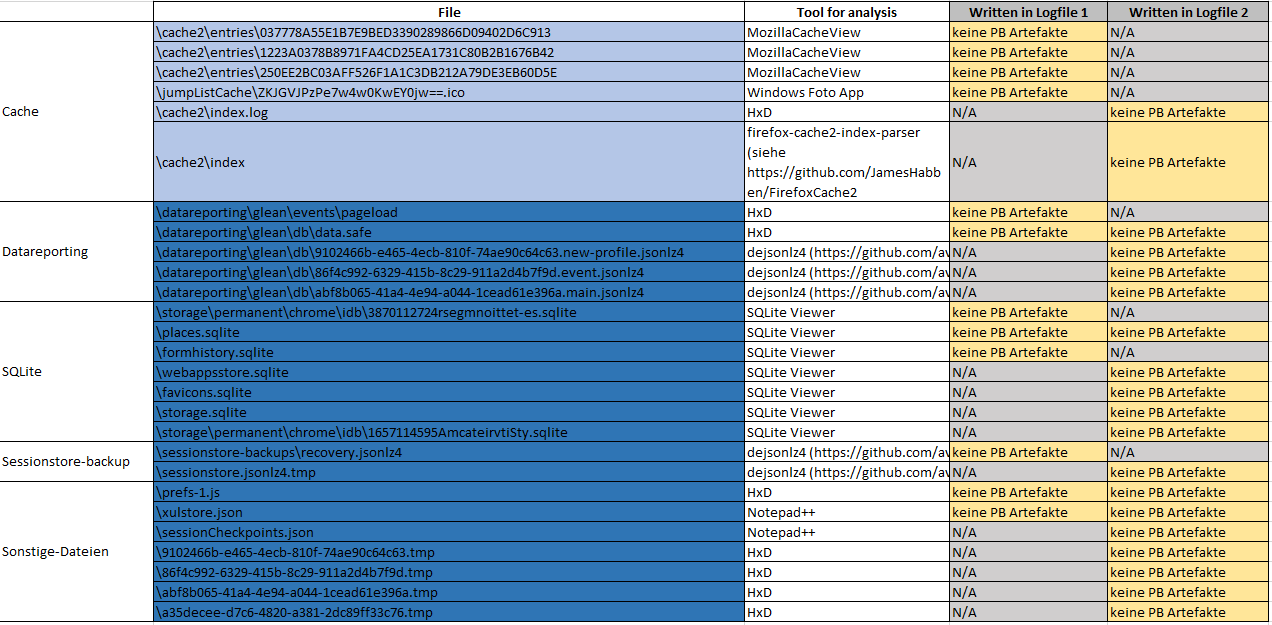
\includegraphics{bilder/firefox-tabelle-logfile1vlogfile2-reduced.png}}
%	\label{...}
	\caption{Tabelle mit wiederherstellbaren Dateien: Logfile 1 vs. Logfile 2}
\end{figure}

Bei detaillierter Untersuchung der Dateien, können zwei Pfade identifiziert werden, in die Firefox während des Versuchs Dateien schreibt. Nur die Dateien in der Cache Kategorie sind im Local Pfad gespeichert.
\begin{itemize}
\item[\textbf{Local}] \texttt{C:$\backslash$Users$\backslash$<User>$\backslash$AppData$\backslash$Local$\backslash$Mozilla$\backslash$Firefox$\backslash$Profiles$\backslash$<Profile>.default-release$\backslash$}
\item[\textbf{Roaming}] \texttt{C:$\backslash$Users$\backslash$<User>$\backslash$AppData$\backslash$Roaming$\backslash$Mozilla$\backslash$Firefox$\backslash$Profiles$\backslash$<Profile>.default-release$\backslash$}
\end{itemize}
In Tabelle X (TODO!) sind die Dateien je nach Speicherort "Local" (Hellblau) oder "Roaming" (Dunkelblau) entsprechend eingefärbt. 

\paragraph*{Cache}
Firefox verwendet den Cache, um Webseiten und deren Ressourcen temporär lokal zu speichern. Dadurch können wiederholte Anfragen an den Server vermieden und die Ladezeiten verringert werden. Die Inhalte dieser Dateien sind binär.
Die Dateien im Format \texttt{$\backslash$cache2$\backslash$entries$\backslash$<ID>} werden dem Cache zugeordnet und im Local Pfad gespeichert.
% https://www.techguy.org/threads/what-exactly-is-in-firefoxs-cache2-folder.1221567/
Wie in Kapitel X beschrieben, können diese Dateien mit dem Tool MZCacheView eingelesen werden.
Wie in Abbildung X gezeigt, konnten im Cache-Ordner im zweiten Snapshot drei JSON Dateien identifiziert werden. Dabei handelt es sich um Zertifikatsdateien, die von der "One Certificate Revocation List" stammen, ein Mechanismus von Firefox zur Überprüfung von Zertifikaten. In keinem der Zertifikate konnten mit HxD private Browsing Artefakte oder besuchte Seiten gefunden werden.
Weiterhin befindet sich im Cache das HTML-Dokument der Firefox Datenschutzseite, welche sich beim ersten Start des Browsers automatisch öffnete. % TODO: Siehe Kapitel X
Weitere Cache Dateien konnten in keinem Snapshot gefunden werden.
\begin{figure}[h!]
	\resizebox{\linewidth}{!}{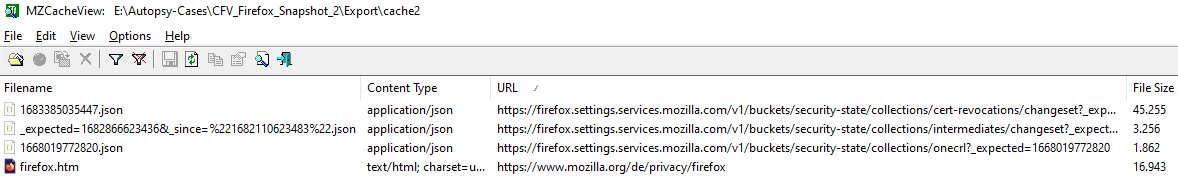
\includegraphics{bilder/firefox-cache.png}}
%	\label{...}
	\caption{Tabelle mit wiederherstellbaren Dateien: Logfile 1 vs. Logfile 2}
\end{figure}
Die Indexdatei \texttt{$\backslash$cache2$\backslash$index} dient als Datenbank im Cache. Sie ermöglicht dem Firefox-Browser, schnell auf die zwischengespeicherten Ressourcen zuzugreifen und diese effizient zu verwalten. Sowohl mit HxD als auch dem Tool FirefoxCache2 konnten keine PB Artefakte identifiziert werden.
*** TODO: Erst in Logfile 2 geschrieben ***

Schließlich enthält die Datei \texttt{$\backslash$jumpListCache$\backslash$ZKJGVJPzPe7w4w0KwEY0jw==.ico} ein $64x64$ Pixel großes Mozilla Logo. Dieses Logo ist keinem Schritt aus dem Browsing Szenario zuzuordnen


\paragraph*{Datareporting}
Dateien im Ordner \texttt{$\backslash$datareporting$\backslash$glean$\backslash$db} sind Teil des Glean-Systems, das für die Sammlung von Telemetriedaten und deren Übermittlung an Mozilla verwendet wird. 
% https://github.com/mozilla/glean
Die Datei \texttt{data.safe.bin} enthält verschlüsselte und anonyme Informationen über die Nutzung des Browsers. In HxD konnten keine keine PB Artefakte gefunden werden
*** TODO: Vergleich Logfile 1 vs 2 ***

Dateien im Foremat \texttt{$\backslash$datareporting$\backslash$glean$\backslash$db$\backslash$<Profilname>.new-profile.jsonlz4} speichern Informationen über das Firefox-Profil, das von Glean verwendet wird. Wie in Kapitel X beschrieben, lassen sich Dateien, im proprietären \textit{jsonlz4}-Format mit dem Tool dejsonlz4 dekomprimieren. Die entstandene JSON Datei wird mit dem Notepad++ JSON Plugin untersucht. Dabei konnten keine PB Artefakte gefunden werden.
*** TODO: Nur in Logfile 2 geschrieben ***

\paragraph*{Sessionstore}
Die Datei \texttt{$\backslash$sessionstore-backups$\backslash$recovery.jsonlz4} enthält eine Sicherungskopie der vorherigen Sitzung. Sie wird erstellt, wenn der Firefox-Browser nach einem Absturz oder einem unerwarteten Beenden neu gestartet wird." % https://support.mozilla.org/de/questions/1221836
Jefferson Scher entwickelte ein Online-Tool zur Analyse von \textit{Sessionstore-Backup} Dateien.
% https://www.jeffersonscher.com/ffu/scrounger.html)
In der Sitzungswiederherstellung konnten wie in Abbildung X gezeigt lediglich die automatisch geöffnete Seite über Firefox Datenschutzhinweise identifiziert werden.
\begin{figure}[h!]
	\resizebox{\linewidth}{!}{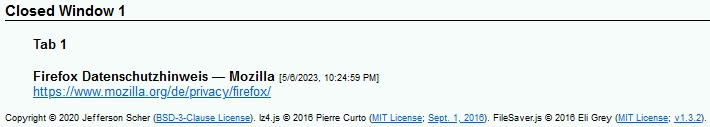
\includegraphics{bilder/firefox-sessionstore.png}}
%	\label{...}
	\caption{Tabelle mit wiederherstellbaren Dateien: Logfile 1 vs. Logfile 2}
\end{figure}
*** TODO: Logfile 1 vs Logfile 2 ***

\paragraph*{Sonstige Dateien}
In der Datei \texttt{prefs-1.js} werden benutzerspezifische Einstellungen und Konfigurationen für den Firefox-Browser gespeichert. Die Datei enthält Präferenzen des Benutzers in Form von JavaScript-Objekten. Es konnten mit HxD keine PB Artefakte gefunden werden.
% https://kb.mozillazine.org/Prefs.js_file
*** TODO: Vergleich Logfile 2 ***

Schließlich speichert die Datei \texttt{xulstore.json} benutzerspezifische Anpassungen und Konfigurationen für den Firefox-Browser. In der Datei konnten mit Notepad++ keine PB Artefakte gefunden werden.
% https://support.mozilla.org/de/kb/firefox-support-troubleshooting-guide
*** TODO: Vergleich Logfile 2 ***	
\subsubsection*{SQLite Datenbänke}
Wie in Kapitel X (Methodik, TODO!) erwähnt, werden SQLite Datenbanken als Datenstrukturen für Nutzerdaten genauer untersucht. Mithilfe der Process Monitor Logfiles wurden die in Tabelle X dargestellten SQLite-Datenbanken für Firefox identifiziert:

\begin{table}[]
\resizebox{\linewidth}{!}{
\begin{tabular}{|l|l|lll}
\cline{1-2}
\textbf{Datenbank}                        & \textbf{Gespeicherte Daten}                                                                                              &  &  &  \\ \cline{1-2}
\textit{places.sqlite}                    & Informationen über Lesezeichen und Verlauf. Zu jeder besuchten Webseite: URL, Seitentitel, Zeitstempel des Besuchs etc.  &  &  &  \\ \cline{1-2}
\textit{cookies.sqlite}                   & Von besuchten Webseiten verwendete Cookies.                                                                              &  &  &  \\ \cline{1-2}
\textit{storage.sqlite}                   & Diverse Webdaten, z. B. Indexed-Datenbanken, Offline-Cache-Daten und andere lokale Speicherinformationen.                &  &  &  \\ \cline{1-2}
\textit{favicons.sqlite}                  & Enhtält Favicons (kleine Symbole in der Adressleiste) um besuchte Webseiten visuell zu identifizieren.                   &  &  &  \\ \cline{1-2}
\textit{webappsstore.sqlite}              & Speichert Informationen über installierte Webanwendungen im Firefox-Browser, z.B. Berechtigungen und Einstellungen.      &  &  &  \\ \cline{1-2}
\textit{1657114595AmcateirvtiSty.sqlite}  & Datenspeicher für Activity Stream, eine personalisierte Übersicht über Browser-Aktivitäten beim Öffnen eines neuen Tabs. &  &  &  \\ \cline{1-2}
\textit{3870112724rsegmnoittet-es.sqlite} & Datenspeicher für Remote Settings, eine zentrale Verwaltung von benutzerspezifischen Browsereinstellungen.               &  &  &  \\ \cline{1-2}
\end{tabular}
}
\end{table}

Jede dieser Datenbanken wurde in allen vier Snapshots miteinander verglichen. Die Dateiextraktion und Dateianalyse erfolgte analog zur Methodik in Kapitel X (TODO!).
Die Ergebnisse wurden in Tabelle X (TODO!) dargestellt.

\begin{figure}[h!]
	\centerline{\resizebox{\linewidth}{!}{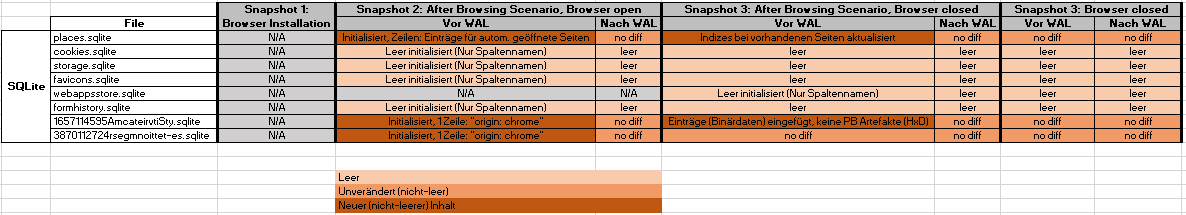
\includegraphics{bilder/firefox-sqlite-table.png}}}
	\label{chart:final-criteria}  
	\caption{Comparison of found PB artifacts between RAM Dumps}
\end{figure}
Nach Browser-Installation (Snapshot 1) existierte noch keine der SQLite-Dateien.

Nach dem Browsing Szenario (Snapshot 2) wurde festgestellt, dass alle SQLite-Datenbanken 
initialisiert wurden, außer \texttt{webappsstore.sqlite}. Dabei wurden in \texttt{places.sqlite} die automatisch im normalen Modus geöffnete Datenschutzhinweise Seite eingetragen. 
In restlichen Datenbanken wurden leer initialisiert, nur die Spaltennamen wurden eingetragen.
Der Inhalt aller erstellten Datenbanken blieb nach Durchführung von PRAGMA WAL Checkpoints unverändert.

Nach Schließen des Browsers (Snapshot 3) wurden in \texttt{places.sqlite} die Indizes bei eingetragenen Seiten aktualisiert. Die SQLite-Datenbank \texttt{1657114595AmcateirvtiSty.sqlite} erhielt ein binäres Datenobjekt als Eintrag. Bei der Untersuchung mit HxD konnten keine Artefakte gefunden werden. Weiterhin wurde \texttt{webappsstore.sqlite} leer initialisiert. Die restlichen Daten blieben im Vergleich mit Snapshot 2 unverändert. Ebenfalls veränderte sich nicht der Inhalt nach Durchführung von PRAGMA WAL Checkpoints.

Nach herunterfahren der VM (Snapshot 4) gab es keine Änderungen in den SQLite Datenbanken, auch nach Durchführung der PRAGMA WAL Checkpoints.
	
Somit wurden in den SQLite Datenbanken von Firefox keine zurückverfolgbaren PB Artefakte im privaten Modus hinterlassen.


Mithilfe des Process Monitors wurde festgestellt, dass sowohl während des Browsing Szenarios (Logfile 1) als auch danach (Logfile 2) Inhalte in Dateien geschrieben wurden. Wie zusammenfassend in Abbildung X (TODO!) dargestellt, wurde mit Ausnahme der Datareporting Dateien gab es in Logfile 1 stets mehr oder genauso viele Schreiboperationen wie in Logfile 2.
Keine Schreiboperation hinterließ jedoch Private Browsing Artefakte.
\begin{figure}[h!]
	\centerline{\resizebox{\linewidth}{!}{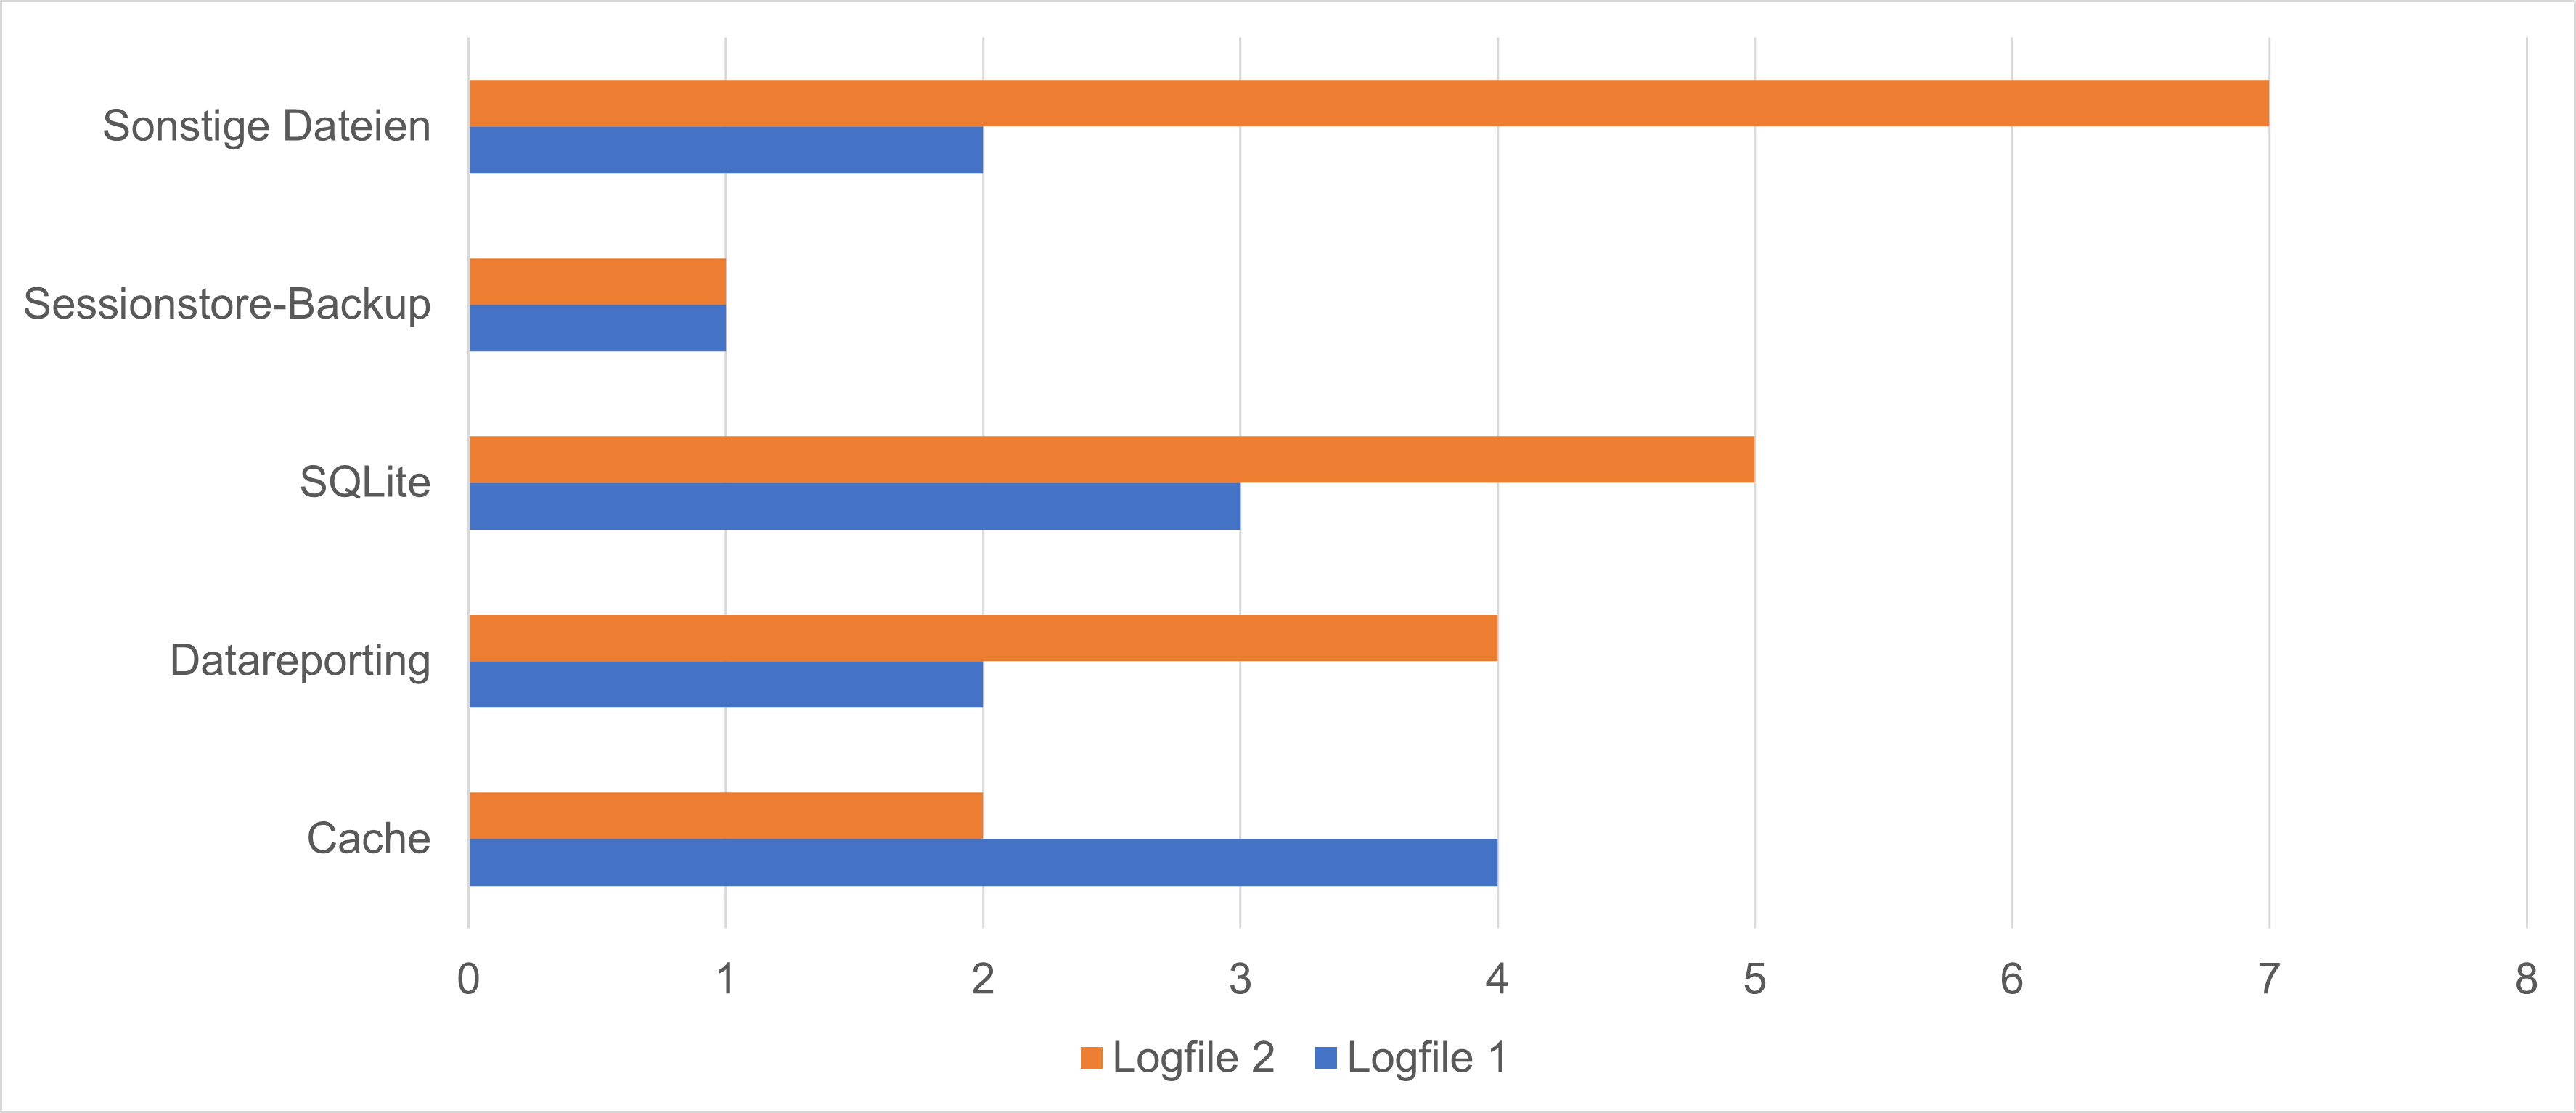
\includegraphics{bilder/bar-chart-logfile1vs2-test.png}}}
	\label{chart:final-criteria}  
	\caption{Comparison of found PB artifacts between RAM Dumps}
\end{figure}


%Literatur:
%	o no traces were found in “common locations” \cite{Montasari.2015}
%		>  “places.sqlite”, “webappsstore. sqlite”, “sessionstore.bak”, “search.json” and “nssckbi.dll”
%	o	Safebrowsing: Alle Dateien in /safebrowsing-updating/ nicht relevant. Dort nur .vlpset und .sbstore Dateien. Speichern 256-Bit Hash von URLs, die auf SafeSearch Blacklist stehen 
%	o	Cache-Dateien: drei Caches: startupCache, jumpListCache (beide enthalten Binärdateien ohne Browsing Artefakte) und cache2 (können mit MozillaCacheView untersucht werden, enthalten keine Browsing Artefakte)
%	o	SQLite Datenbanken: Sqlite Dateien erst ohne WAL Dateien untersuchen, Danach mit sqlite3 Konsole: WAL in Datenbank schreiben mit: PRAGMA wal\_checkpoint; places.sqlite besonders relevant, da dort Browser in public Modus Browsing URLs verwaltet (Am besten hier vergleich mit Public Browsing machen)	
%		> \cite{Fayyad.2021} for Mozilla Firefox, 7 database files were recovered: cookies.sqlite-shm, places.sqlite-shm, prefs.js etc.
%		> \cite{Muir.2019} The two SQLite databases used by Firefox to track cookies and history (cookies.sqlite und places.sqlite) were both recoverable from the file system after deletion	
%		Ergebnisse stehen im Gegensatz zu \cite{Hedberg.2013} :
%			o	Chrome und Firefox: Einträge in places.sqlite + history.sqlite DB gefunden während PB! (Noch aktuell??)
%		Sonderfall: SQlite DB-Crash \cite{Hedberg.2013}
%			> WAL Files/Journal Files bei Crash gefunden -> Kann genutzt werden um zu beweisen, dass privater Browser genutzt wurde
%			> Daher: WAL Rollback mit sqlite3	
%	o	Jsonlz4 \& balkz4: Enthalten komprimierte Firefox-Sessions, jsonlz4 Dateien können mit Tool "entkomprimiert" werden: https://www.jeffersonscher.com/ffu/scrounger.html

\subsection*{Uncommon Locations}

Nachfolgend werden die Analyseergebnisse der Firefox Uncommon Locations beschrieben.
Wie in Kapitel X erläutert, wird im Gegensatz zu Common Locations die Suchrichtung umgekehrt und es werden alle gesammelten Daten nach einem spezifischen PB Artefakt durchsucht.
Somit benötigt ein Forensiker kein Wissen über das Browserverhalten. Stattdessen wird sich auf die Vollständigkeit der Funktionen von Forensik-Tools verlassen. Im Rahmen dieses Versuchs werden die Tools Autopsy und Volatility verwendet.

\subsubsection*{Analyse mit Autopsy}

Bei den Common Locations in Kapitel X wird Autopsy nur zur Dateiextraktion genutzt. Im Falle der Uncommon Locations dient Autopsy als forensisches Werkzeug zur Datenanalyse.

Eine Autopsy Stichwortsuche gemäß Methodik in Kapitel X (TODO!) lieferte in allen Snapshots keine Treffer. Es wurde zusätzlich das \texttt{\$Carved} Verzeichnis durchsucht, in dem Autopsy alle wiederhergestellten Dateien speichert.

Anschließend wurden die automatisch von Autopsy kategorisierten Dateien untersucht. Gemäß Methodik in Kapitel X wurden dazu die Dateien der Kategorien "Web Bookmarks", "Web Cookies", "Web History" sowie "Web Categories" analysiert.
Beim Vergleich der Festplattenabbilder wurde festgestellt, dass ein Snapshot stets die kategoriesierten Dateien des vorherigen Snapshots enthielt. Es sind innerhalb einer Kategorie nur neue Dateien dazugekommen. Somit enthält Snapshot 4 in jeder Kategorie alle Dateien der vorherigen Snapshots.

\paragraph*{Web Bookmarks}

Bereits vor Durchführung des Browsing Szenarios enthielt Firefox im ersten Snapshot die Bing Startseite als gespeichertes Leesezeichen. In den restlichen Snapshots 2 -- 4 blieb diese Kategorie unverändert.

\begin{figure}[h!]
	\centerline{\resizebox{\linewidth}{!}{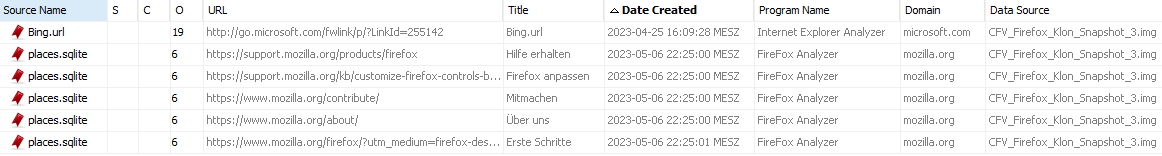
\includegraphics{bilder/cfv_firefox_autopsy_web_bookmarks.png}}}
	\label{chart:final-criteria}  
	\caption{Autopsy Web Bookmarks}
\end{figure}

\paragraph*{Web Cookies}
Auch diese Kategorie enthält bereits vor Beginn des Browsing Szenarios zehn Cookie-Einträge in der Datei \texttt{WebCacheV01.dat}. Dabei handelt es sich um eine Datenbank des Microsoft Edge Browsers zur Speicherung von Nutzerdaten. Diese Datei verhält sich ähnlich wie die in diesem Versuch relevanten SQLite-Dateien. Die Datei enhält. Bei den Einträgen handelt es sich um Cookies für Bing und die Outlook Webseite, obwohl diese Seiten nie in Microsoft Edge geöffnet wurden. In den Snapshots 2 -- 4 kamen keine weiteren Einträge in dieser Kategorie hinzu.
\begin{figure}[h!]
	\centerline{\resizebox{\linewidth}{!}{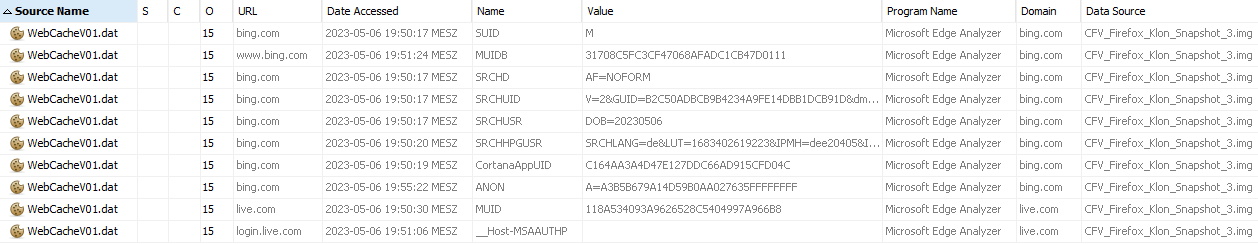
\includegraphics{bilder/cfv_firefox_autopsy_web_cookies.png}}}
	\label{chart:final-criteria}  
	\caption{Autopsy Web Cookies}
\end{figure}

\paragraph*{Web History}
Diese Kategorie listet alle Dateien mit gespeichertem Suchverlauf auf. Vor Beginn des Browsing Szenarios (Snapshot 1) enthält die Kategorie ebenfalls zwei Einträge zur Outlook Webseite in der Datei \texttt{WebCacheV01.dat}. Nach Durchführung des Browsing Szenarios (Snapshot 2) wurde ein Eintrag in der \texttt{places.sqlite} Datenbank hinzugefügt. Dabei handelt es sich um die automatisch im normalen Browsingmodus geöffnete Firefox-Standardseite über Datenschutzhinweise. Dies deckt sich mit den Beobachtungen der Common Locations in Kapitel X. Darüber hinaus enthält dieser Snapshot für die Datei \texttt{WebCacheV01.dat} den Eintrag \texttt{file:///Z:/Logfile\_1}. Dabei handelt es sich um das Process Monitor Logfile, das gemäß Methodik in Kapitel X (TODO!) über den gemeinsamen VM-Ordner zum Analyse-Rechner transportiert wurde. Ergänzt wird das in Snapshot 3 durch den Eintrag \texttt{file:///Z:/Logfile\_2}, dem zweiten Process Monitor Logfile. In Snapshot 4 werden in dieser Katgeorie keine neuen Dateien erfasst.
\begin{figure}[h!]
	\centerline{\resizebox{\linewidth}{!}{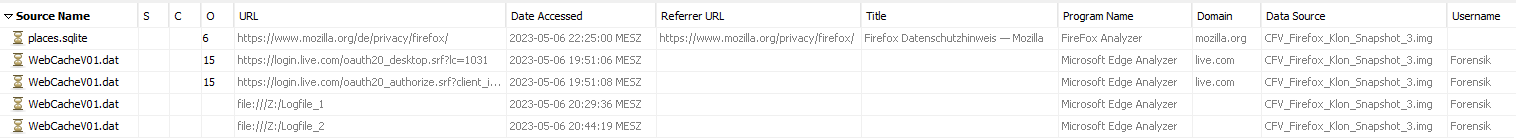
\includegraphics{bilder/cfv_firefox_autopsy_web_history.png}}}
	\label{chart:final-criteria}  
	\caption{Autopsy Web History}
\end{figure}

\paragraph*{Web Categories}
Diese Kategorie klassifiziert im Speicherabbild gefundene Browsing Artefakte nach Inhalt.
Vor Beginn des Browsing Szenarios (Snapshot 1) werden hier bereits zwei Einträge aufgelistet. Der Eintrag \texttt{bing.com} wird als "Suchmaschine" klassifiziert und \texttt{live.com} als "Web-Email".
Wie oben erwähnt, wurden beide Seiten nie aufgerufen. Es gab keine zusätzlichen Einträge in dieser Kategorie in den Snapshots 2 bis 4.
\begin{figure}[h!]
	\centerline{\resizebox{\linewidth}{!}{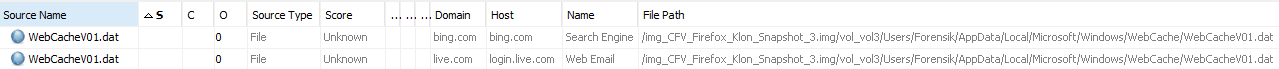
\includegraphics{bilder/cfv_firefox_autopsy_web_categories.png}}}
	\label{chart:final-criteria}  
	\caption{Autopsy Web Categories}
\end{figure}
		

Somit wurden in allen Kategorien ausschließlich Browsing Artefakte des Edge Browsers in der Datei \texttt{WebCacheV01.dat} gefunden, sowie ein Eintrag in der Firefox SQLite Datenbank \texttt{places.sqlite}. Die eingetragene Firefox-Standardseite deckt sich mit den Ergebnissen der Common Locations in Tabelle X. Die aufgelisteten Einträge in der Datei \texttt{WebCacheV01.dat} sind nicht auf Schritte des Browsing Szenarios zurückzuführen. Die Einträge sind bereits im ersten Snapshot enthalten, obwohl vor Beginn des Browsing Szenarios keine Browseraktivitäten durchgeführt wurden. Weiterhin enthölt diese Datei Einträge über die Process Monitor Logfiles, welche über einen gemeinsamen VM-Ordner zum Rechner transportiert wurde, auf dem die virtuelle Maschine läuft.
In keiner der Kategorien konnten private Browsing Artefakte identifiziert werden.

%Literatur:
%	o	Autopsy Keywortsuche: 
%		>	In alles Snapshots ergebnislos (keine Keyword-Hits
%		-->	In Literatur: Autoren fanden Ergebnisse in pagefile.sys 
%			> Autopsy: websites and some of the keywords found in hidden file called “pagefile.sys” \cite{Mahlous.2020}
%			o \cite{Montasari.2015} traces were found in: 
%				> However, on investigating the “pagefile.sys”, some entries were discovered
%				> Using the “data carving” technique, profile picture was recovered
%			o \cite{Said.2011} 
%				> Examining pagefile.sys showed some positive hits 			
%		--> Evtl. hier zeigen, was gefunden werden kann, wenn RAM reduziert
%		--> Aber auf Problem hinweisen, dass gefundener String in pagefile nicht direkt Browser zugeordnet werden kann
%		> \cite{Gabet.2018}	Firefox only produced three recoverable artefacts as reported by both tools (FTK, Autopsy) --> Artefakte werden nicht genannt!
%		> \cite{Muir.2019} Autopsy Keyword Suche nach Suchbegriffen: unallocated space
%		> Autopsy Carving Module (\$Carved): \cite{Muir.2019}
%			•	When searching for the string ’clot’ from the browsing protocol, six .dll, .edb and .reg files were discovered in unallocated space.
%			•	Further searching of unallocated space uncovered references to the Tor installation directory and the obfs4 bridging IP addresses
%			•	browsing data found in NTUSER.DAT was also replicated in unallocated space.
%	o	Autopsy PlugIns:
%		>	*** TODO: Hier Liste mit PlugIns ***

\subsubsection*{Analyse mit Volatility}
Nachdem die Firefox Festplattenabbilder als Uncommon Location mit Autopsy untersucht wurden, werden nachfolgend die Analyseergebnisse des RAMs als Uncommon Location beschrieben. 
Dazu wurde eine Stringsuche im gesamten RAM nach PB Artefakten durchgeführt.
Wie in Kapitel X ausführlich beschrieben muss ein gefundener String eindeutig einem Browser zugeordnet werden können. 

Deshalb wurde dazu das Volatility PlugIn "Yarascan" verwendet, ein Werkzeug um nach bestimmten Mustern im RAM zu suchen. Dazu wurden die in Tabelle X aufgeführten Yara-Regeln verwendet.
Wie in Kapitel Methodik (TODO!) beschrieben, wird davon ausgehend das PlugIn "pslist" verwendet, um den Prozessnamen anhand PID zu identifizieren.
Die Ergebnisse dieser Stringsuche sind nachfolgend nach Kategorie geordnet.

\paragraph*{Yararule HTML}
In keinem der Firefox RAM Dumps wurden HTML Fragemente der besuchten Seiten gefunden. Somit wird diese Yara-Regel nicht weiter betrachtet.

\paragraph*{Yararule Keyword}
Wie in Abbildung X (TODO!) gezeigt, wurden alle Suchbegriffe "pfaffenhofen", "nanoradar", "mooserliesl" sowie "mallofamerica" identifiziert im zwiten RAM Dump, nach dem Browsing Szenario mit geöffnetem Browser, identifiziert. Die Artefakte befinden sich ausschließlich im zweiten RAM Dump. Die Suchbegriffe wurden größtenteils in den Speicherbereichen von Firefox-Prozessen gefunden. Nur in zwölf Fällen wurden Suchbegriffe in anderen Prozessen identifiziert. Am häufigsten wurde der Suchbegriff "pfaffenhofen" mit 1301 gefundenen Artefakten im zweiten Firefox RAM Dump gefunden. Dies ist vermutlich auf den Google Maps Kartenbereich zurückzuführen, einen visuellen Ausschnitt der Karte, welcher bei der Google-Suche erscheint und Informationen über die geografische Lage, Straßen, Sehenswürdigkeiten und andere relevante Orte in der gesuchten Stadt zeigt. In den RAM Dumps 1 und 3 konnten Artefakte zu den Suchbegriffen identifiziert werden.
\begin{figure}[h!]
	\centerline{\resizebox{\linewidth}{!}{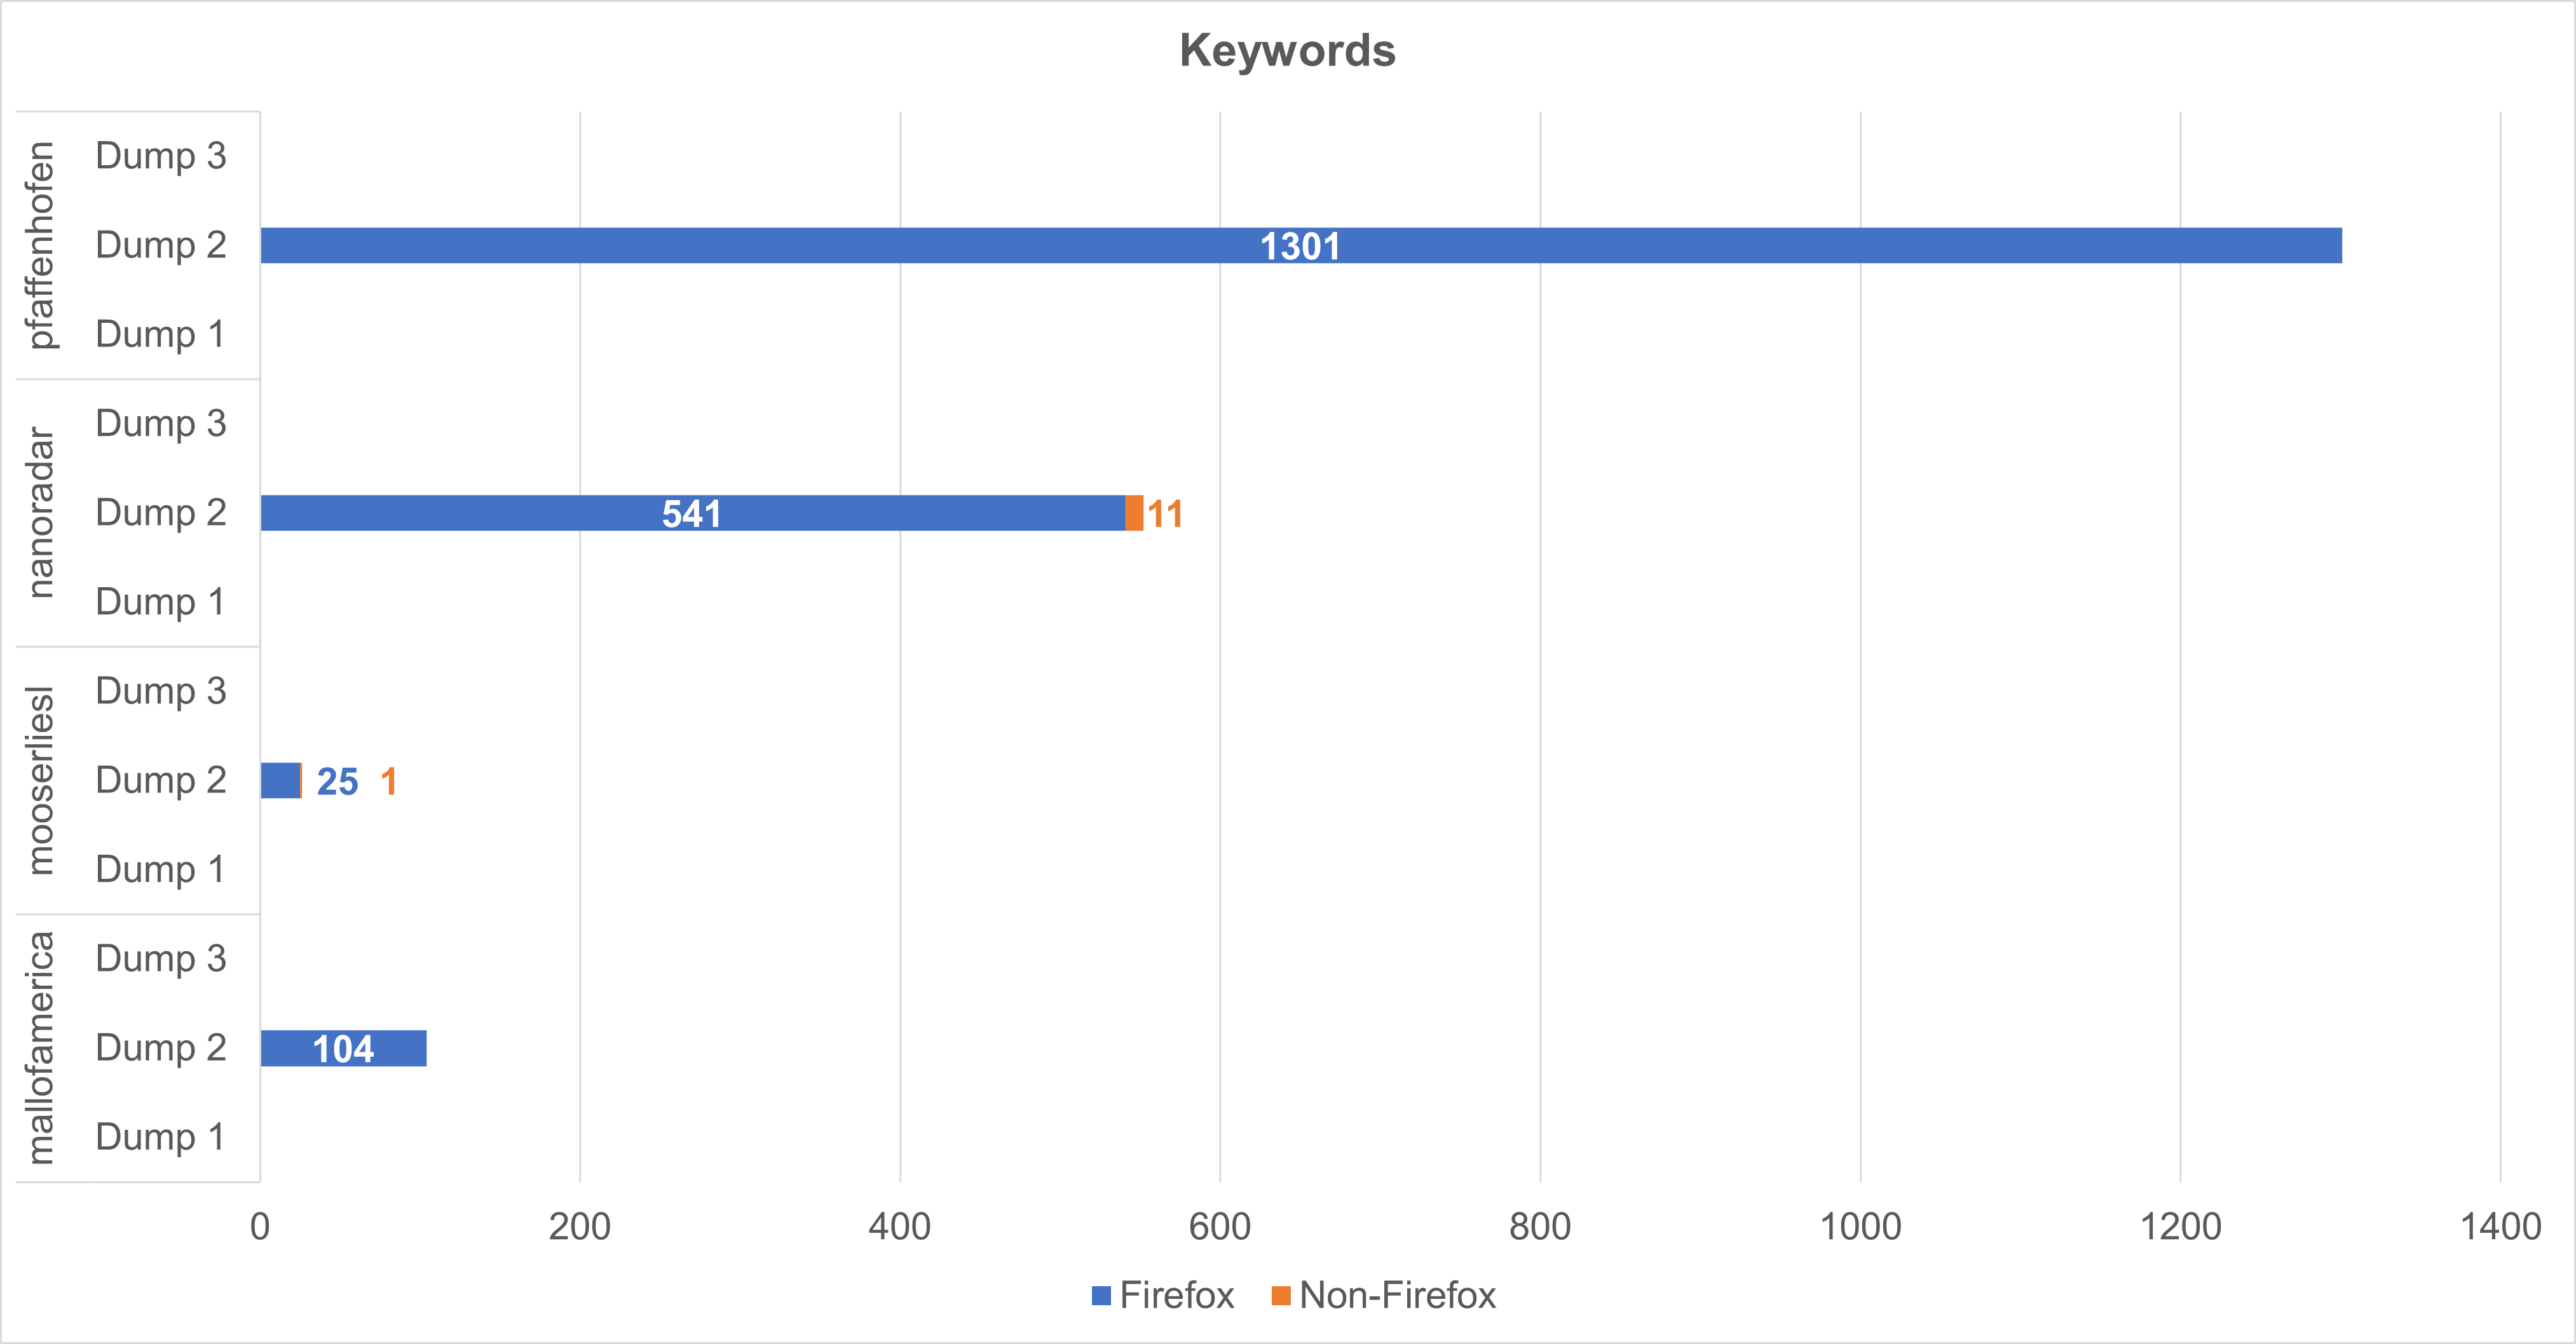
\includegraphics{bilder/volatility/firefox/keywords.png}}}
	\label{chart:final-criteria}  
	\caption{Keywords}
\end{figure}

\paragraph*{Yararule URL}
\begin{figure}[h!]
	\centerline{\resizebox{\linewidth}{!}{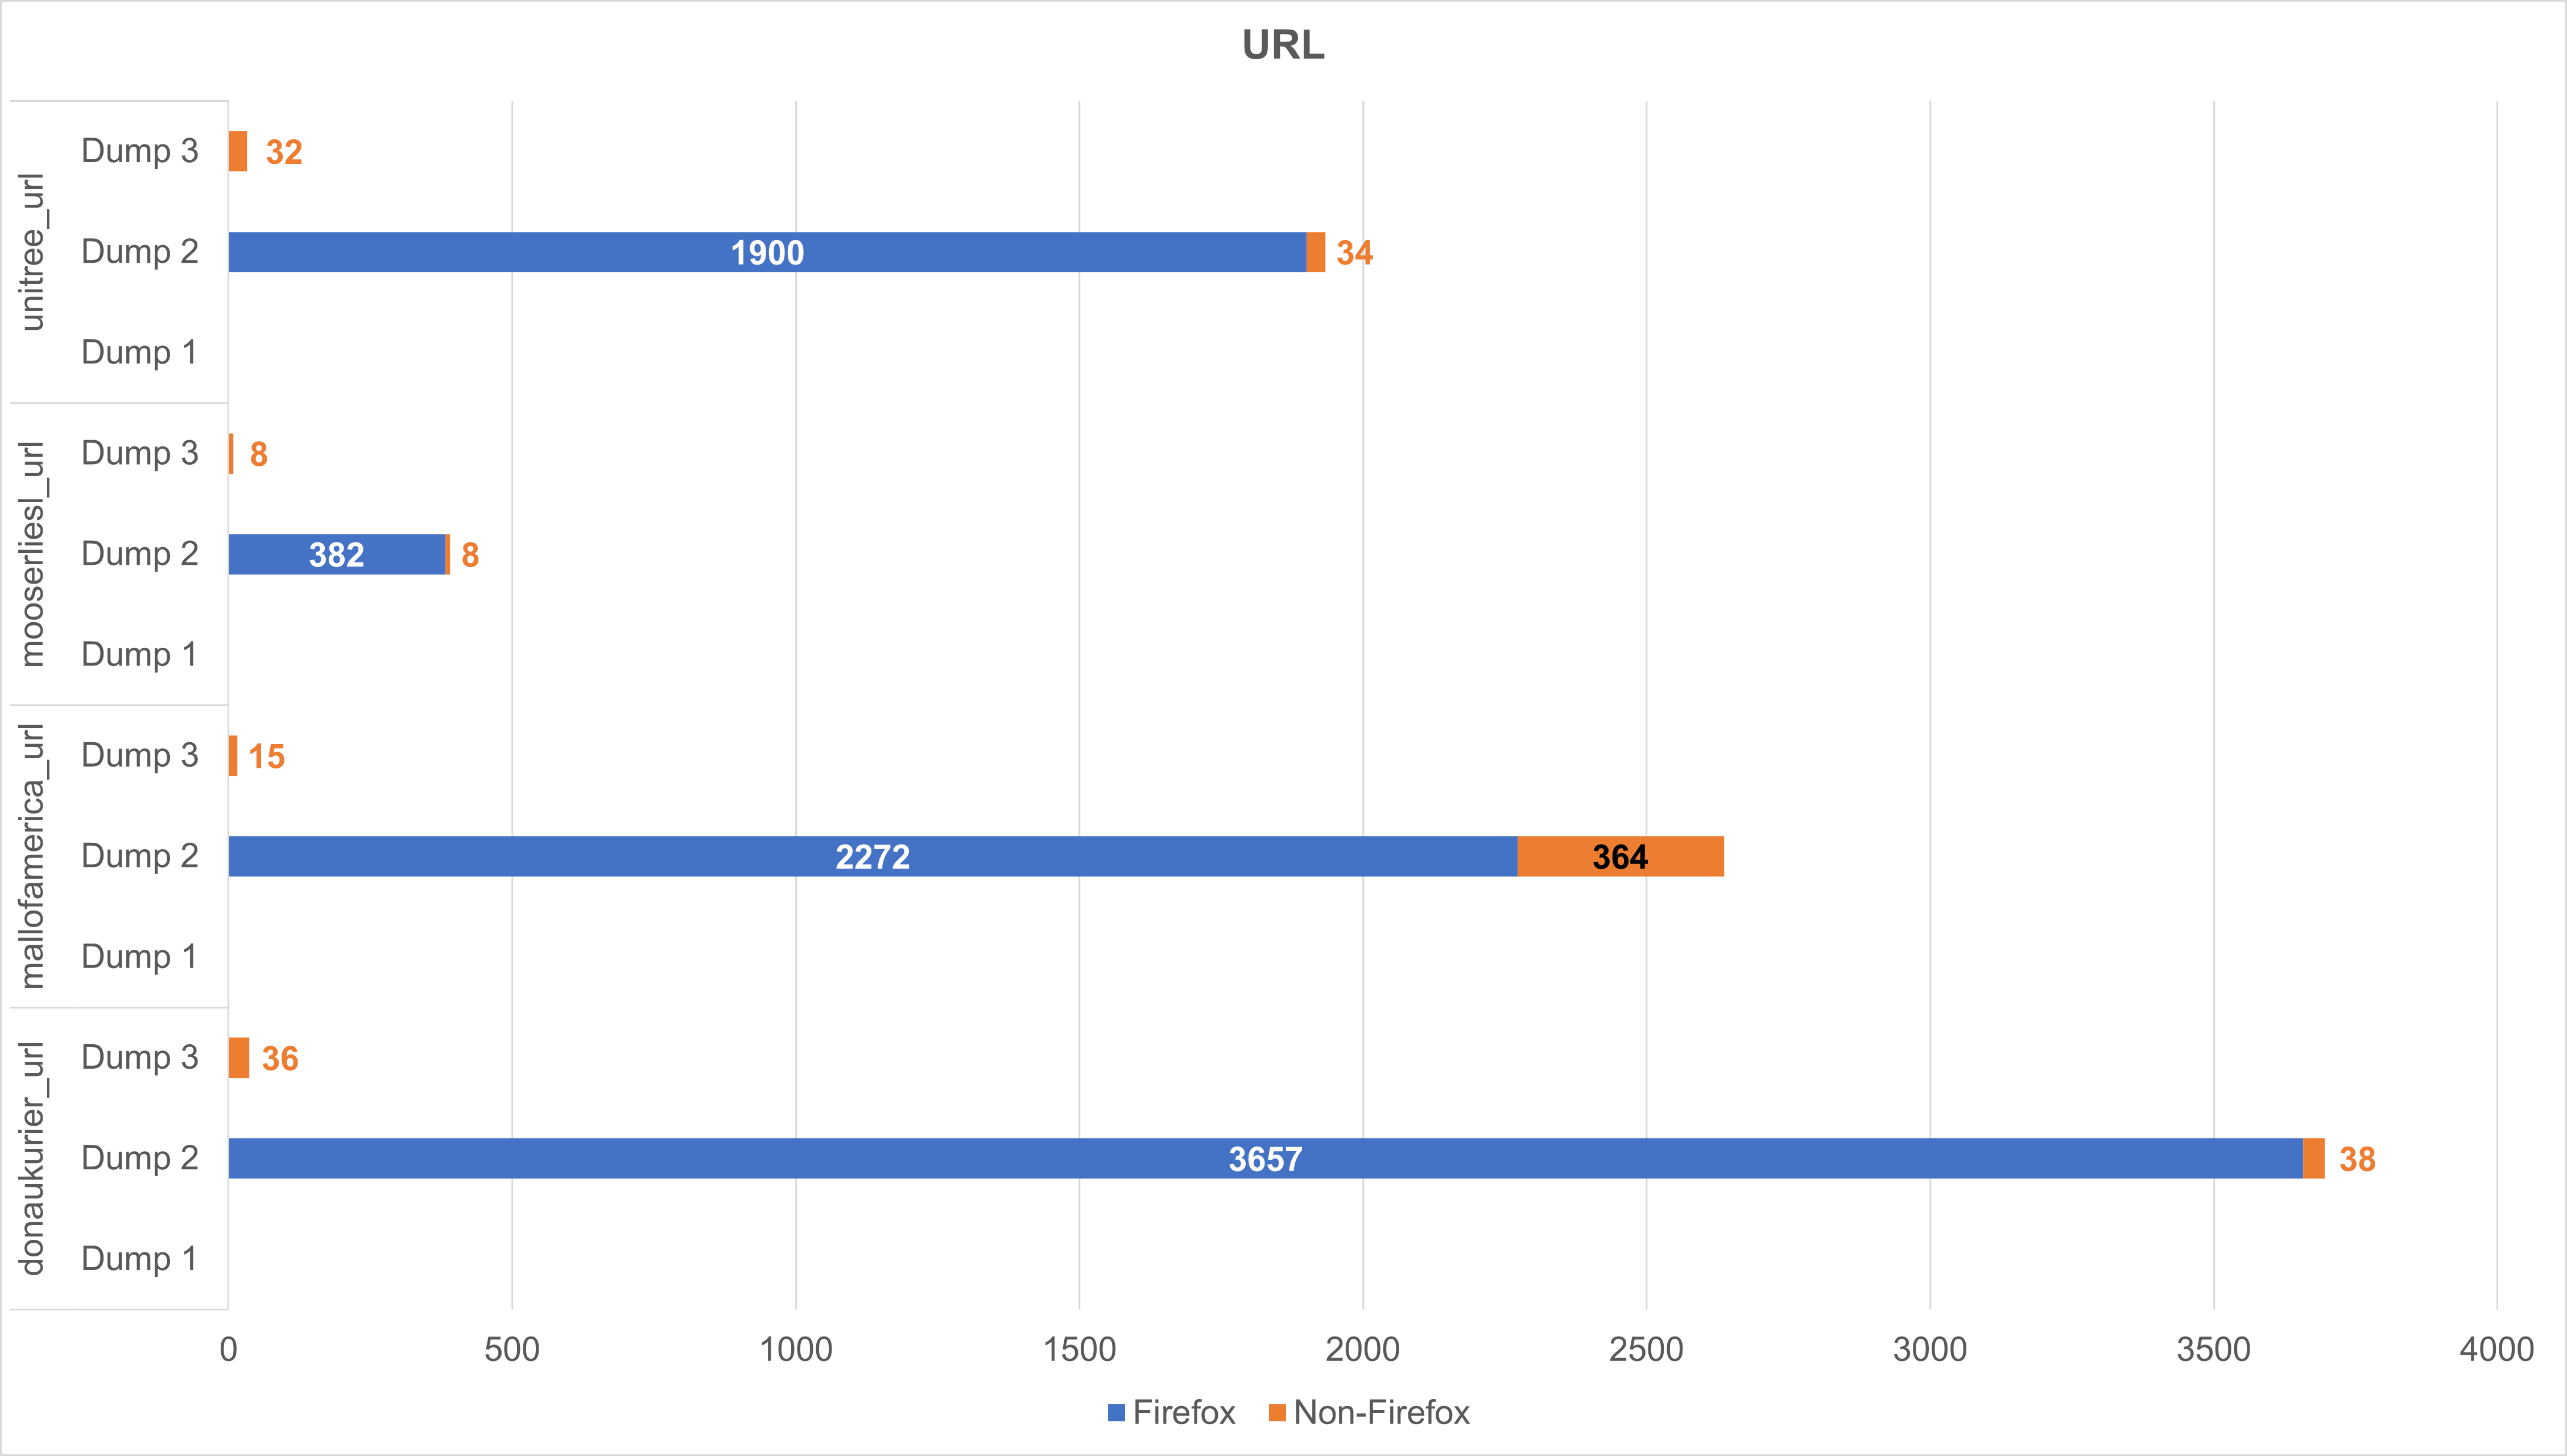
\includegraphics{bilder/volatility/firefox/url.png}}}
	\label{chart:final-criteria}  
	\caption{URL}
\end{figure}
Es konnten in den Arbeitsspeicherabbildern alle besuchten URLs unitree.com, mooserliesl.de, mallofamerica.com sowie donaukurier.de identifiziert werden.
Dabei wurden die meisten Artefakte nach dem Browsing Szenario mit geöffnetem Browser (RAM Dump 2) gefunden. Alle besuchten URLs wurden in diesem Dump sowohl in Firefox als auch anderen Prozessen gefunden, wobei die meisten Artefakte in Firefox Prozessen zu finden sind. Dabei wurde "mooserliesl.de" mit insgesamt 390 Artefakten am wenigsten gefunden, "donaukurier.de" mit über 3600 Artefakten am häufigsten.

Bemerkenswert ist, dass URL Artefakte gefunden wurden, nachdem der Browser geschlossen wurde (RAM Dump 3). Dabei wurde kein URL Artefakte in einem Firefox Prozess gefunden.
Anhand der PID $2252$ wurde festgestellt, dass sich alle URL Artefakte des dritten RAM Dumps in einem "svchost.exe" Prozess mit der gleichen PID befinden. Unter dem "Service Host" Prozess laufen gruppierte Windows-Dienste, um Ressourcen zu sparen und die Systemleistung zu verbessern.
Volatility bietet das Plugin "svcscan" an, mit dem alle laufenden Dienste ausgegeben werden können.
Bei Anwendung auf den dritten RAM Dump wurde jedoch zu keinem Dienst eine PID angegeben, wordurch der Dienst mit den URL Artefakten nicht im RAM identifiziert werden konnte. 
% https://learn.microsoft.com/de-de/windows/application-management/svchost-service-refactoring
Stattdessen wurde der dritte Snapshot aufgetaut, um im laufenden Windowsbetrieb den Dienst mithilfe des Process Explorers zu identifizieren.
Wie in Abbildung X (TODO!) gezeigt, wurde anhand der PID $2252$ der Dienst "DNSCache" ermittelt.
\begin{figure}[h!]
	\centerline{\resizebox{\linewidth}{!}{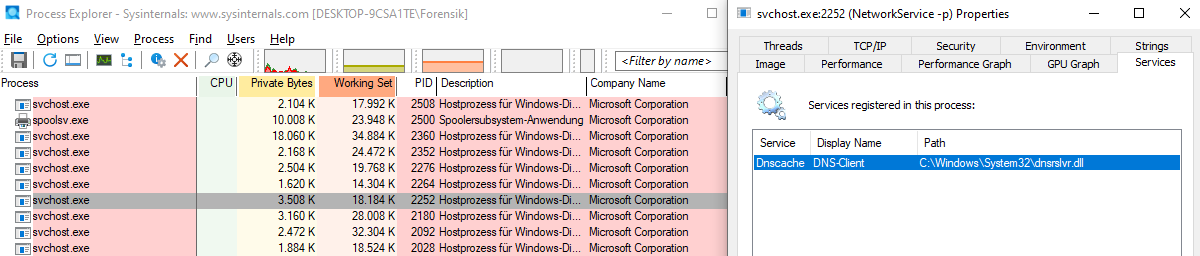
\includegraphics{bilder/firefox-dnscache.png}}}
	\label{chart:final-criteria}  
	\caption{URL}
\end{figure}
Der DNSCache-Dienst unter Windows ist ein Teil des Betriebssystems, der für die Übersetzung von Domainnamen in IP-Adressen verantwortlich ist. Der DNSCache-Dienst speichert DNS-Anfragen und Antworten temporär, umd wiederholte DNS-Anfragen zu beschleunigen.
% https://learn.microsoft.com/en-us/answers/questions/47441/how-to-disable-windows-10-dns-cache-services
Nach Löschen des DNSCaches mit dem Kommandozeilenbefehl \texttt{ipconfig /flushdns}, dem Schließen aller Process Monitor Instanzen sowie Beenden des DNSCaches Services wurde erneut ein RAM-Dump durchgeführt. Dort wurden keine URL Artefakte mehr gefunden.

\paragraph*{Yararule Mail}
\begin{figure}[h!]
	\centerline{\resizebox{\linewidth}{!}{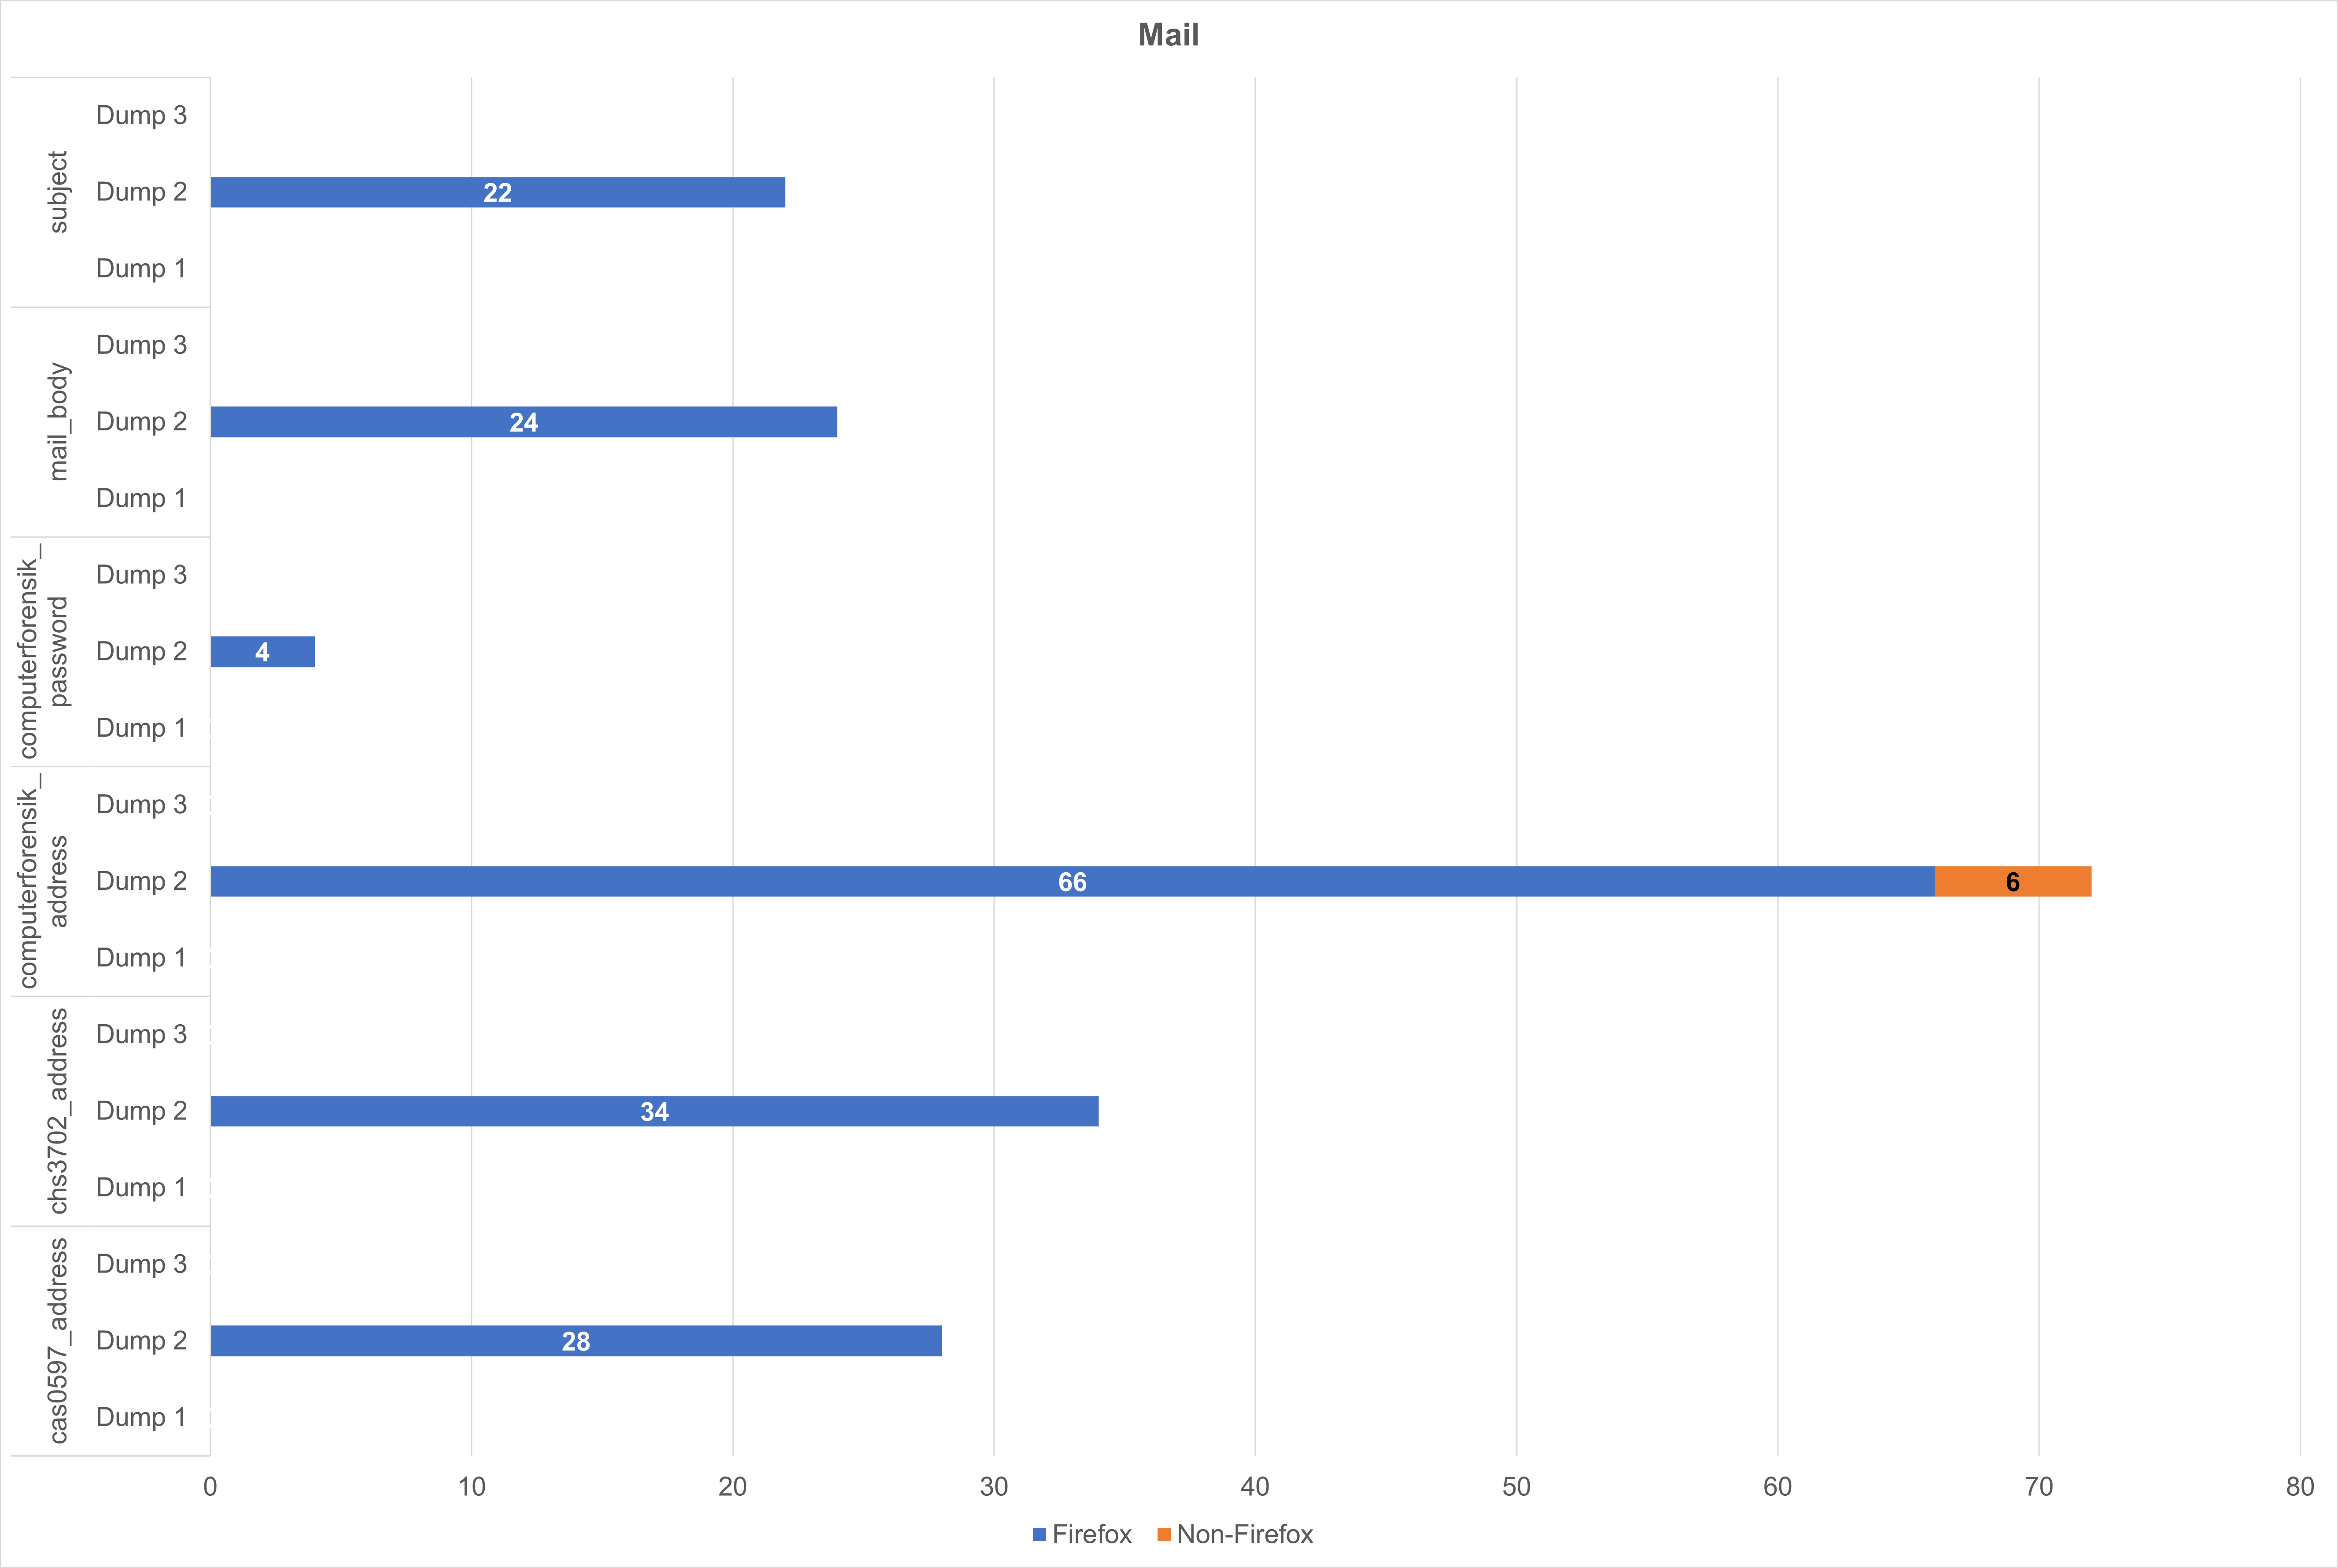
\includegraphics{bilder/volatility/firefox/mail.png}}}
	\label{chart:final-criteria}  
	\caption{Mail}
\end{figure}
Es konnten alle E-Mail Artefakte des Browsing Szenarios gefunden werden.
Die Artefakte befinden sich ausschließlich im zweiten Firefox RAM Dump, nach dem Browsing Szenario mit geöffnetem Browser.
Unter den gefundenen Artefakten befindet sich mit zwölf Vorkommen am häufigsten die Absenderadresse "computerforensikvl@gmail.com". Dieses Artefakt wurde als einziges Mail-Artefakt in anderen Prozesses außer Firefox gefunden.

Bemerkenswert ist, dass das Passwort des Google-Accounts, mit dem die E-Mails verschickt wurden, vier mal als Klartext im RAM gefunden wurden. Das Passwort wurde in je zwei Firefox Prozessen mit den PIDs 7420 und 8424 zwei mal gefunden. Tabelle X zeigt die virtuellen Speicheradressen der Artefakte aus der Yarascan Ausgabe.
\begin{table}[]
\resizebox{\linewidth}{!}{
\begin{tabular}{|c|c|c|ll}
\cline{1-3}
\textbf{Virtuelle Speicheradresse} & \textbf{PID} & \textbf{Byte-Offset in extrahierter Speicherseite} &  &  \\ \cline{1-3}
0xb9ce29180c8                      & 7420         & 0x11dd40c8                                         &  &  \\ \cline{1-3}
0x2859f4ffd4e0                     & 7420         & 0x12e234e0                                         &  &  \\ \cline{1-3}
0x24083b41858                      & 8424         & 0x583858                                           &  &  \\ \cline{1-3}
0x240840e5b08                      & 8424         & 0x96bb08                                           &  &  \\ \cline{1-3}
\end{tabular}
}
\end{table}

Zu diesen Artefakten wurde gemäß Methodik in Kapitel X der String Kontext -- die Zeichen vor und nach dem gefundenen Artefakt im Speicherbereich -- ermittelt. Dazu wurde gemäß Methodik in Kapitel X mithilfe des Volatility memmap-Plugins die Abbildung der virtuellen Speicheradressen auf den Byte-Offset in der extrahierten Speicherseite des Prozesses ermittelt. 
\begin{figure}[h!]
	\centerline{\resizebox{0.7\linewidth}{!}{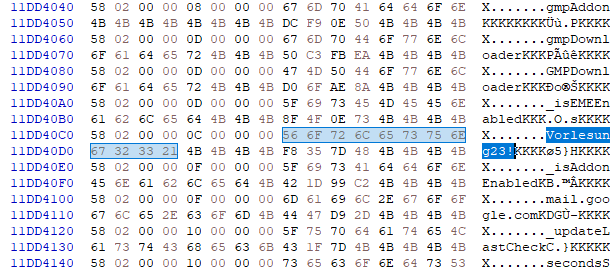
\includegraphics{bilder/volatility/firefox/password_0xb9ce29180c8_7420.png}}}
	\label{chart:final-criteria}  
	\caption{Password in memory page of PID 7420 at Byte-Offset 0x11dd40c8}
\end{figure}
Wie in Abbildung X gezeigt, sind in der Speicherseite des Prozesses mit PID $7420$ konnte vor und nach dem gefundenen Passwort am Byte-Offset $0xb9ce29180c8$ neben der Gmail-Url "mail.google.com" Code-Fragmente der "Gecko-Engine" zu finden. Dieser Teil des Firefox Browsers ist für das Rendering von Webinhalten verantwortlich, einschließlich HTML, CSS, JavaScript und anderen Medienformaten wie Bildern, Audio und Video.
% https://wiki.mozilla.org/GeckoMediaPlugins
\begin{figure}[h!]
	\centerline{\resizebox{0.7\linewidth}{!}{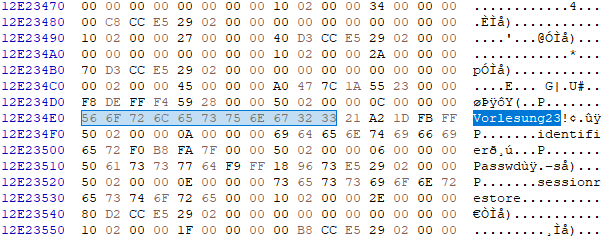
\includegraphics{bilder/volatility/firefox/password_0x2859f4ffd4e0_7420.png}}}
	\label{chart:final-criteria}  
	\caption{Password in memory page of PID 7420 at Byte-Offset 0x12e234e0}
\end{figure}
In der gleichen Datei konnte nach dem gefundenen Passwort am Byte-Offset $0x24083b41858$ die Strings "Passwd" sowie "sessionrestore" (siehe Common Location "Sessionstore" in Kapitel X) identifiziert werden. 
Wie in den Abbildungen X und Y (TODO!) gezeigt, können in den Byte-Offsets der gefundenen Passwörter in der Speicherseite der PID 8424 konnten kein Kontext ermittelt werden. Im Gegensatz zur Speicherseite der PID 7420 wird das Passwort dort mit 2 Bytes pro Zeichen enkodiert. Das eine Unicode-Zeichenenkodierung vermuten.
\begin{figure}[h!]
	\centerline{\resizebox{0.7\linewidth}{!}{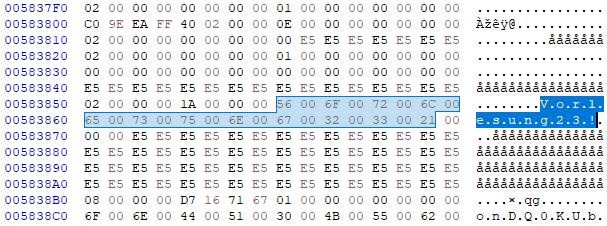
\includegraphics{bilder/volatility/firefox/password_0x24083b41858_8424.png}}}
	\label{chart:final-criteria}  
	\caption{Password in memory page of PID 8424 at Byte-Offset 0x583858}
\end{figure}
\begin{figure}[h!]
\centerline{\resizebox{0.7\linewidth}{!}{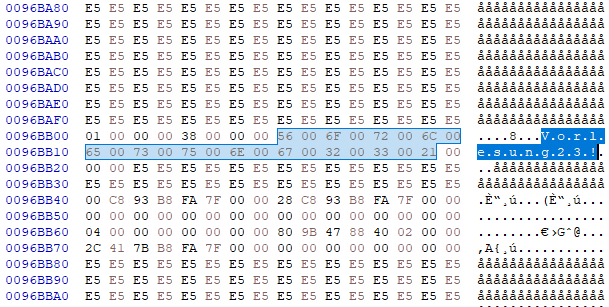
\includegraphics{bilder/volatility/firefox/password_0x240840e5b08_8424.png}}}
\label{chart:final-criteria}  
\caption{Password in memory page of PID 8424 at Byte-Offset 0x96bb08}
\end{figure}
				
\paragraph*{Yararule Image}
Das im Browsing Szenario geöffnete Donaukurier Logo wurde ausschließlich im zweiten RAM Dump in drei mal in Firefox Prozessen gefunden.
\begin{figure}[h!]
	\centerline{\resizebox{\linewidth}{!}{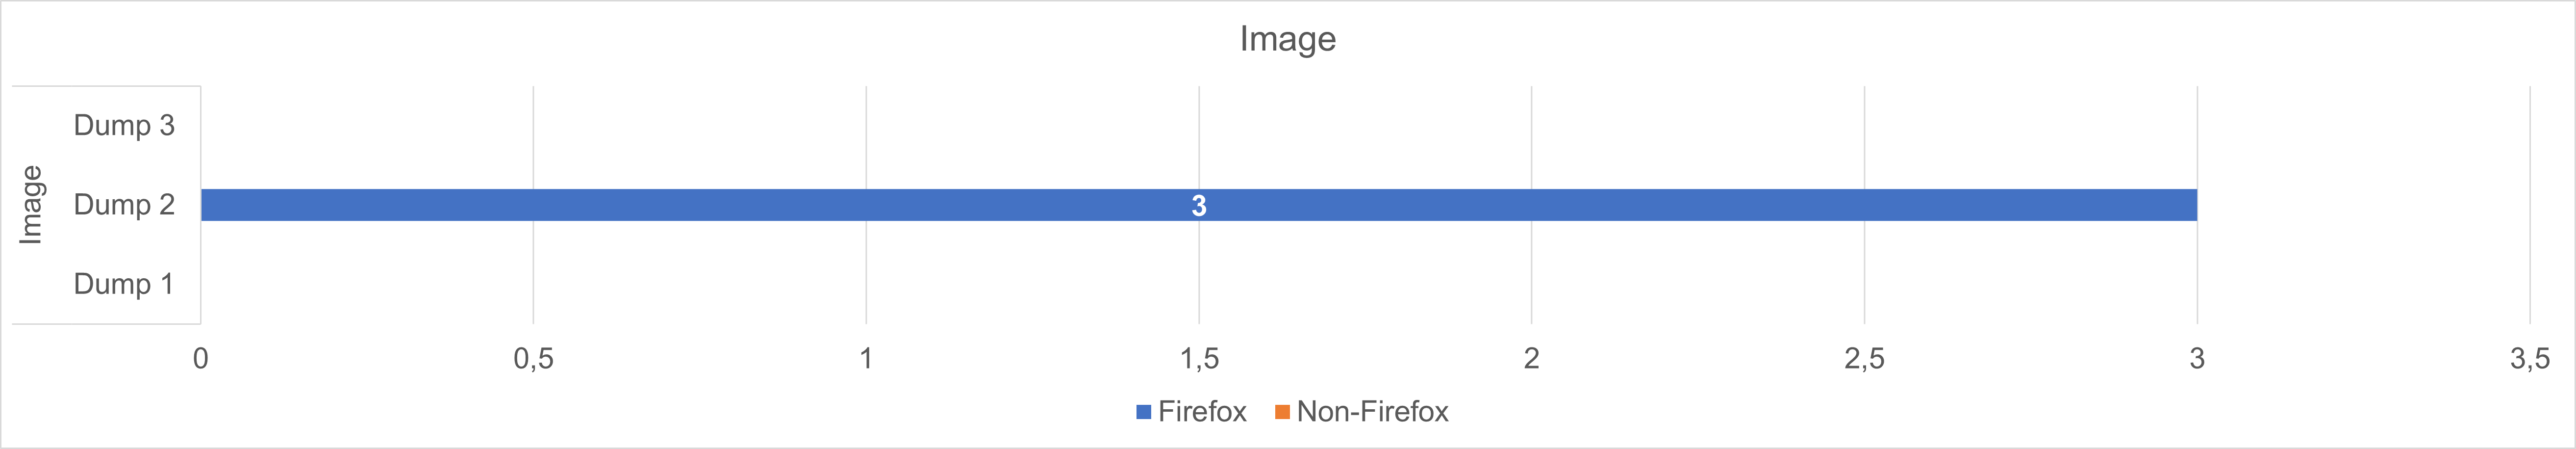
\includegraphics{bilder/volatility/firefox/image.png}}}
	\label{chart:final-criteria}  
	\caption{Image}
\end{figure}

Wie in Abbildung X zusammenfassend gezeigt wurden vor dem Browsing Szenario, keine private Browsing Artefakte im ersten RAM Dump gefunden.
Nach dem Browsing Szenario mit geöffnetem Browser konnten die meisten Artefakte identifiziert werden. Dabei wurden am häufigsten URL Artefakte in Firefox Prozessen gefunden. Zudem konnte hier das E-Mail Passwort im Klartext lokalisiert werden.
Nach Schließen des Browsers konnten im dritten Snapshots URLs im DNSCache Windows Service gefunden werden. Nach leeren des Caches und Beenden des DNSCache Services konnten wurden keine Artefakte gefunden.
\begin{figure}[h!]
	\centerline{\resizebox{\linewidth}{!}{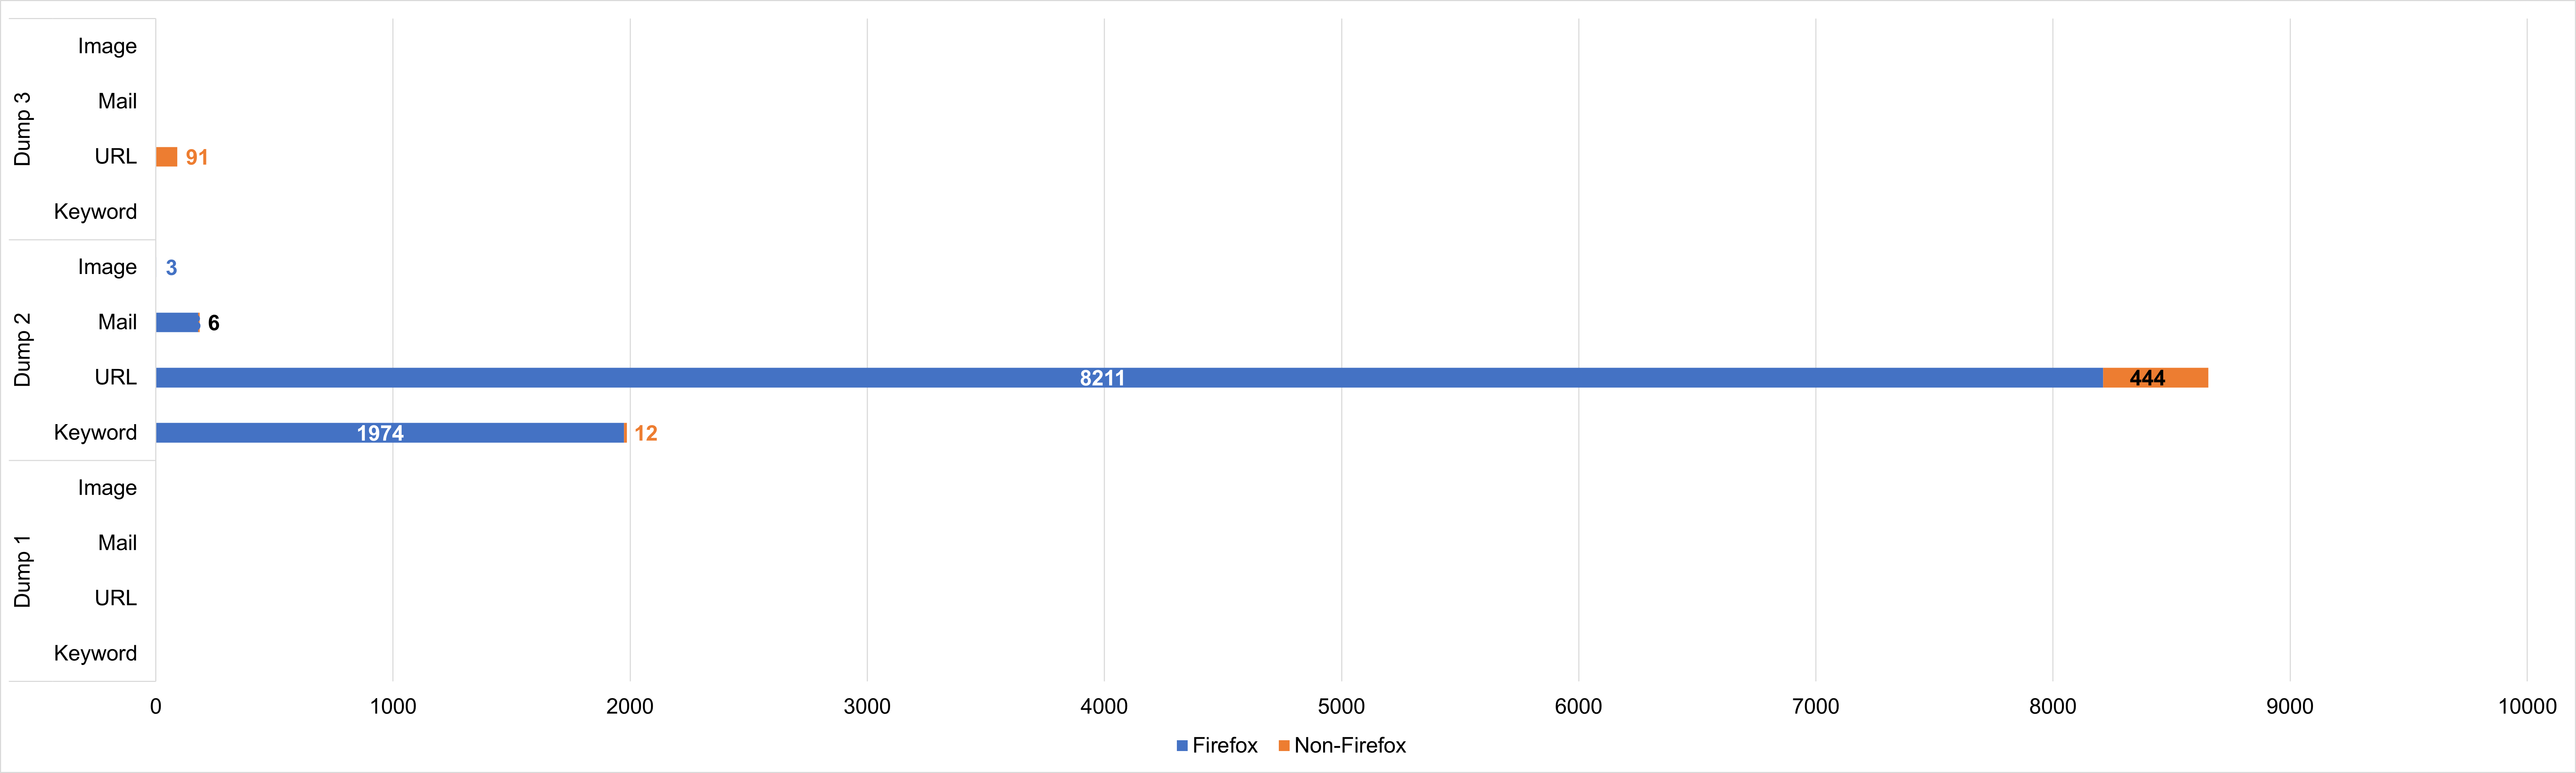
\includegraphics{bilder/volatility/firefox/summary.png}}}
	\label{chart:final-criteria}  
	\caption{Summary}
\end{figure}


\subsection*{Registry}

Die Analyse der Registry zählt gemäß Methodik in Kapitel X sowohl zu den Common als auch Uncommon Locations 

\subsubsection*{Process Monitor SetValue Operations}

Als Teil der Common Locations werden für Firefox alle Registry "SetValue" Schreiboperationen der beiden Process Monitor Logfiles untersucht.

In beiden Logfiles wurden zwei Kategorien von Registry Keys geschrieben: "PreXULSkeletonUISettings" und "Business Activity Monitoring". In Abbildung X ist der Anteil der Schreiboperationen je Kategorie für beide Logfiles gezeigt.
\begin{figure}[h!]
	\centerline{\resizebox{\linewidth}{!}{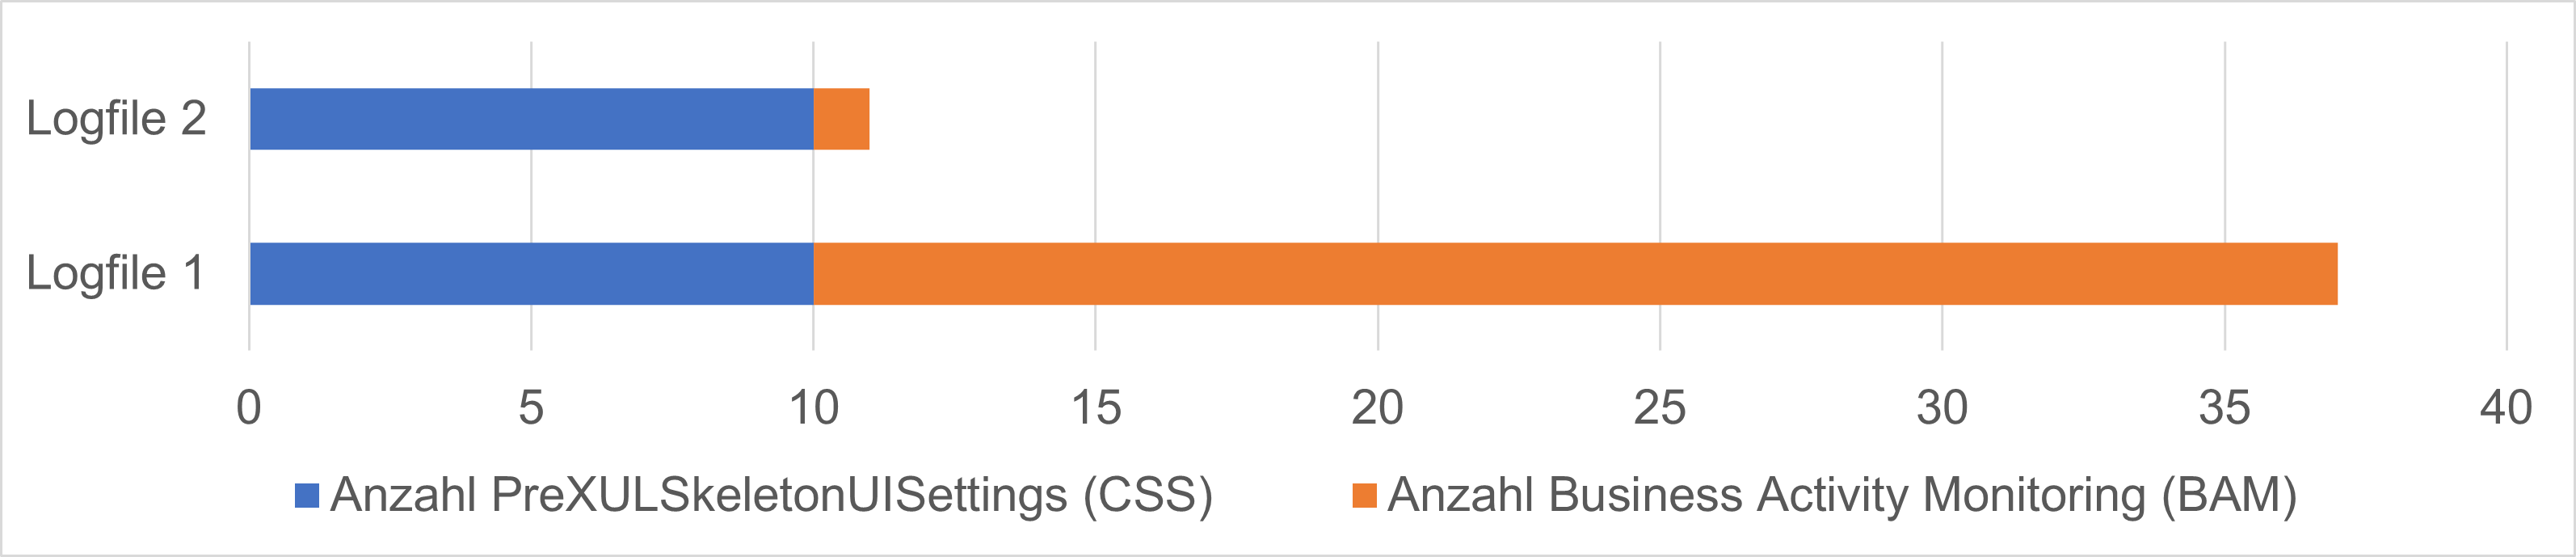
\includegraphics{bilder/firefox-registry-stacked-bar-chart.png}}}
	\label{chart:final-criteria}  
	\caption{Comparison of found PB artifacts between RAM Dumps}
\end{figure}

\paragraph*{PreXULSkeletonUISettings}
%https://itigic.com/skeleton-ui-new-firefox-interface-to-start-up-much-faster/#google_vignette
Der "PreXULSkeletonUISettings" Registry Key enthält Einstellungen für die Benutzeroberfläche (UI) des Firefox-Browsers, insbesondere für das sogenannte "Skeleton UI, eine vereinfachte Benutzeroberfläche, die während des Ladens des Browsers angezeigt wird, bevor die vollständige Benutzeroberfläche geladen ist. 
PreXULSkeletonUISettings Registry Keys haben das Format \texttt{HKCU$\backslash$SOFTWARE$\backslash$Mozilla$\backslash$Firefox$\backslash$PreXULSkeletonUISettings$\backslash$<Absoluter Firefox Installationspfad>$\backslash$firefox.exe|<Skeleton UI Setting>}.
Somit enthält der Key den absoluten Installationspfad von Firefox gefolgt von einer Skeleton UI Einstellung. Nachfolgend sind alle möglichen UI Einstellungen aufgelistet, gefolgt vom Datentyp des Keys.
\begin{itemize}
	\item ScreenX (DWORD)
	\item ScreenY (DWORD)
	\item Width (DWORD)
	\item Height (DWORD)
	\item Maximized (DWORD)
	\item Flags (DWORD)
	\item CssToDevPixelScaling (REG\_BINARY)
	\item UrlbarCSSSpan (REG\_BINARY)
	\item SearchbarCSSSpan (REG\_BINARY)
	\item SpringsCSSSpan (REG\_BINARY)
\end{itemize}
Somit enthalten die Keys nur Daten zur Formatierung und Struktur der grafischen Oberfläche. Es wurden keine PB Artefakte geschrieben

\paragraph*{Business Activity Monitoring}
"Business Activity Monitoring", kurz BAM ist eine weitgehend undokumentierte Windows Funktion, die im Hintergrund ausgeführte Programme steuert.
Der Registry Key hat das Format \texttt{HKLM$\backslash$System$\backslash$CurrentControlSet$\backslash$Services$\backslash$bam$\backslash$State$\backslash$UserSettings$\backslash$<SID>$\backslash$Device$\backslash$HarddiskVolume2$\backslash$<Absoluter Firefox Installationspfad>$\backslash$firefox.exe} und den Datentyp REG\_BINARY.
Jeder Schlüssel wird durch die Sicherheits-ID (SID) des Benutzers identifiziert.
Ein BAM Registry Key schreibt für alle ausgeführten Programme --- hier Firefox --- den Zeitstempel der letzten Ausführung.
PB Artefakte sind dabei nicht enthalten.
% https://learn.microsoft.com/de-de/biztalk/core/business-activity-monitoring-bam
% https://notes.qazeer.io/dfir/windows/_artefacts_overview 

\subsubsection*{Stringsuche in Registry Hives}

Gemäß Methodik in Kapitel X wird die Firefox Registry als Uncommon Location behandelt, indem über alle auf der Festplatte vorhandenen Registry Datenbanken, den Registry-Hives, eine Stringsuche durchgeführt wird, ohne die Struktur der Hives zu beachten. 
Dazu wurden sowohl die System-Hives als auch die User-Hives aus Tabelle X (TODO!) aus jedem Snapshot extrahiert und mithilfe des Registry Explorers nach PB Artefakten durchsucht.
Dabei wurde in keinem Snapshot in keinem Hive ein PB Artefakt gefunden.

%Literatur:
%	>	Auf Autor verweisen: angeblich in Shellactivities Ergebnisse. --> Nicht mehr vorhanden in aktueller Version (Verweis auf E-Mail)
%	>	Process Monitor/Regshot zeigen keine relevanten Key-Änderungen
%	> \cite{Muir.2019}: Autopsy Keyword Suche nach Suchbegriffen: Ergebnisse in \%SystemRoot\%Minidump NTUSER.DAT, ntuser.dat.LOG1 (a log of changes to NTUSER.DAT)
%	> Zentral: shellactivites Key:	NTUSER.DAT --> “shellactivities” key \cite{Muir.2019}
%	> \cite{Rochmadi.2017} Detection of registry changes helps to determine what the appropriate plugin is used to search for digital evidence using volatility memory forensic:
%	- RegQueryValue:	HKCU/Software/Microsoft/Windows/CurrentVersion/InternetSettings/Connections/DefaultConnectionSettings
%	- RegCloseValue: 	HKCU/Software/Microsoft/Windows/CurrentVersion/InternetSettings/Connections
%	- IRP\_MJ\_READ: C:/pagefile.sys


*** TODO: Zusammenfassung Firefox ***


\newpage


% ######################################################################
% ######################################################################
% ######################################################################
% ######################################################################


\section{Tor}

In diesem Abschnitt werden die Ergebnisse der Datenanalyse der Common Locations, Uncommon Locations sowie der Registry für den Tor-Browser präsentiert.

\subsection*{Common Locations}

Als Erstes werden die Common Locations analysiert, um potenzielle Hinweise auf Internetaktivitäten des Browsing Szenarios zu finden. Bei der Untersuchung der gängigen Speicherorte wird gemäß der im Kapitel X (TODO!) beschriebenen Methodik zwischen Schreibvorgängen in den Protokolldateien des Process Monitors und den SQLite-Datenbanken zur Verwaltung von Benutzerdaten unterschieden.

\subsubsection*{Process Monitor WriteFile Operations}

Bei der Versuchsdurchführung für den Tor-Browser gemäß Kapitel X wurden drei Process Monitor Logfiles erstellt.
Diese Dateien enthalten alle aufgezeichneten Prozessaktivitäten während des Browsing Szenarios, nach dem Erzeugen einer "Neuen Identität" sowie nach Schließen des Browsers.
Eine gemäß Methodik in Kapitel X verarbeitete Tabelle mit allen in den Logfiles identifizierten Dateien ist im Anhang X aufgeführt.
Für jede Datei wurde vermerkt ob und wie sie wiederherstellbar war, mit welchem Tool die Datei analysiert wurde und ob PB Artefakte enthalten sind.

In Tabelle X (TODO!) sind die ausschließlich wiederherstellbaren Dateien aufgeführt.
Die Dateien wurden in die vier Kategorien "Cache", "datareporting", und "Sonstige Dateien" eingeordnet.
In keiner der identifizierten Dateien konnten PB Artefakte gefunden werden.

\begin{figure}[h!]
	\resizebox{\linewidth}{!}{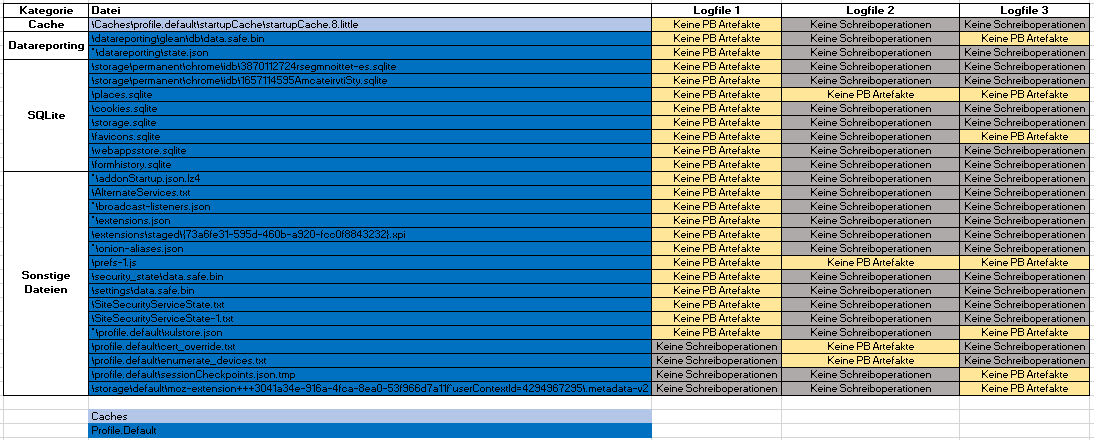
\includegraphics{bilder/tor-tabelle-logfile1vlogfile2vlogfile3-reduced.png}}
%	\label{...}
	\caption{Tabelle mit wiederherstellbaren Dateien: Logfile 1 vs. Logfile 2}
\end{figure}

Ähnlich wie bei der Analyse der Schreiboperationen von Firefox in Kapitel X (TODO!), konnten für den Tor-Browser zwei Pfade identifiziert werden, wo sich Dateien befinden, in die geschrieben wurde.
\begin{itemize}
\item[\textbf{Caches}] \texttt{C:$\backslash$Users$\backslash$Forensik$\backslash$Desktop$\backslash$Tor Browser$\backslash$Browser$\backslash$TorBrowser$\backslash$Data$\backslash$Browser$\backslash$Caches$\backslash$profile.default$\backslash$}
\item[\textbf{Profile.default}] \texttt{C:$\backslash$Users$\backslash$Forensik$\backslash$Desktop$\backslash$Tor Browser$\backslash$Browser$\backslash$TorBrowser$\backslash$Data$\backslash$Browser$\backslash$profile.default$\backslash$}
\end{itemize}
In Tabelle X (TODO!) sind die Dateien je nach Speicherort "Caches" (Hellblau) oder "Profile.default" (Dunkelblau)  eingefärbt. 

Bei der Auswertung der Process Monitor Logfiles wurde festgestellt, dass alle Schreibopertationen von "firefox.exe" Prozessen durchgeführt wurde, nicht "tor.exe" 

Obwohl keine der Dateien PB Artefakte enthält, werden zum vollständigen Browserverständnis im Sinne der White-Box-Forensik die wichtigsten Dateien im Zusammenhang des Tor-Browsers genauer untersucht.


\paragraph*{Cache}
Der Tor-Browser schreibt eine einzige Cache-Datei \texttt{$\backslash$Caches$\backslash$profile.default$\backslash$startupCache$\backslash$startupCache.8.little} im Caches-Pfad. Alle anderen geschriebenen Dateien befinden sich im "Profile.default"-Pfad.
Die Datei "startupCache.8.little" ist eine interne Datei, welche erstellt wird, um den Startvorgang des Browsers zu beschleunigen. Sie enthält Informationen über bereits geladene Browser-Komponenten wie JavaScript-Code, CSS-Dateien, Bilder und andere Ressourcen.  %https://wiki.mozilla.org/StartupCache
Bei Untersuchung mit HxD konnten keine PB Artefakte gefunden werden.

\paragraph*{Datareporting}
Im "Datareporting"-Ordner wird vom Tor-Browser die Datei \texttt{$\backslash$datareporting$\backslash$data.safe.bin} geschrieben. Sie enthält verschlüsselte und anonyme "Glean" Informationen über die Nutzung des Browsers. % https://github.com/mozilla/glean
In HxD konnten keine keine PB Artefakte gefunden werden.
Weiterhin wird die Datei \texttt{$\backslash$datareporting$\backslash$state.json} geschrieben
Sie enthält Informationen über den Zustand und die Konfiguration des Tor-Browsers, beispielsweise installierte Add-Ons, oder Browser-Einstellungen. Sie wird verwendet, um dem Browser bei Bedarf den Zustand und die Einstellungen wiederherzustellen."
% https://github.com/mozilla/firefox-data-store-docs/blob/master/README.md
Eine Analyse mit Notepad++ und dem JSON-Plugin brachte keine PB-Artefakte.

\paragraph*{Sonstige Dateien}
Die im ersten Logfile geschriebene Datei \texttt{AlternateServices.txt}
enthält onion URLs des HTTP Alternative Services ist ein Mechanismus. Dieser ermöglicht es Servern, Clients mitzuteilen, dass der Dienst, auf den sie zugreifen, an einem anderen Netzwerkstandort oder über ein anderes Protokoll verfügbar ist. Die Datei speichert diese Zuordnung.
% https://support.mozilla.org/en-US/questions/1310302

Weiterhin wird währen des Browsing Szenarios die Datei \texttt{$\backslash$extensions$\backslash$staged$\backslash${73a6fe31-595d-460b-a920-fcc0f8843232}.xpi} geschrieben. Dabei handelt es sich um das von Tor verwendete "NoScript"-AddOn zur selektiven Ausführung von JavaScript Webseiteninhalten.
Nach Extraktion dieser Datei, kann diese per Drag-and-Drop in ein geöffnetes Firefox-Fenster gezogen werden und es ist möglich, die Erweiterung zu installieren.

Die geschriebene Datei \texttt{onion-aliases.json} enthält "SecureDrop" Adressen, beispielsweise für die Süddeutsche Zeitung.  %https://www.sueddeutsche.de/projekte/kontakt/#securedrop)
SecureDrop ist ein Open-Source-Softwaretool, das von Journalisten und Nachrichtenorganisationen verwendet wird, um anonyme Informationen von Whistleblowern entgegenzunehmen. Es ermöglicht den sicheren Austausch von Informationen, ohne die Identität der Quelle preiszugeben. Whistleblower können über .onion-URLs auf die SecureDrop-Websites zugreifen und vertrauliche Dokumente oder Nachrichten sicher und anonym übermitteln.

%	> % \security_state\data.safe.bin
%		Zweck: The file containing the updated security data % (https://bbs.archlinux.org/viewtopic.php?pid=1952286#p1952286)

Schließlich wurde in die Datei \texttt{SiteSecurityServiceState.txt} geschrieben.
Diese Datei speichert Daten wie Zertifikate, Verschlüsselungseinstellungen und andere Sicherheitsmerkmale, die von den besuchten Websites verwendet werden.
Es ist anzumerken, dass diese Datei früher private Browsing Artefakte enthielt % https://gitlab.torproject.org/tpo/applications/tor-browser/-/issues/18589
. In der akutellen Tor-Browser-Version konnten keine private Browsing Artefakte gefunden werden.
	
\subsubsection*{SQLite Datenbänke}
			Wie in Kapitel X (Methodik, TODO!) erwähnt, werden SQLite Datenbanken als Datenstrukturen für Nutzerdaten genauer untersucht. Mithilfe der Process Monitor Logfiles wurden die in Tabelle X dargestellten SQLite-Datenbanken für Firefox identifiziert:		
 
Aus Process Monitor Logfiles ist erkennbar, dass Tor die gleichen SQLite Datenbanken wie Firefox aus Kapitel X (TODO!) verwaltet und beschreibt.
			
Wie bei der Analyse der SQLite-Datenbanken bei Firefox wird die Entwicklung von Dateiinhalt in allen fünf Festplatten-Images der Snapshots 1, 2, 3-1, 3-2 und 4 betrachtet. Die Ergebnisse sind in Tabelle X (TODO!) dargestellt.
\begin{figure}[h!]
	\centerline{\resizebox{\linewidth}{!}{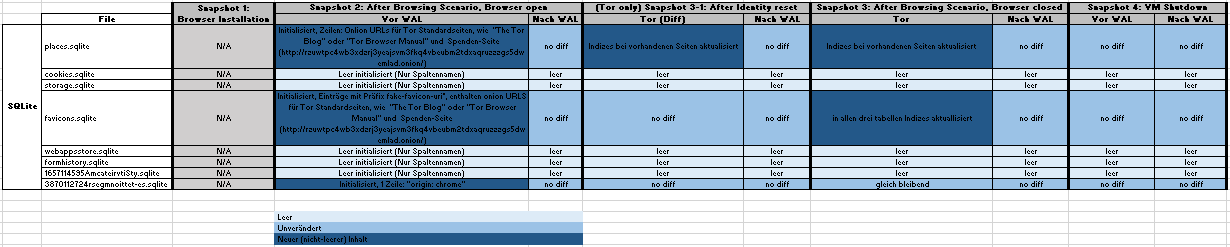
\includegraphics{bilder/tor-sqlite-table.png}}}
	\label{chart:final-criteria}  
	\caption{Comparison of found PB artifacts between RAM Dumps}
\end{figure}
Nach Browser-Installation wurde noch keine SQLite-Datei angelegt (Snapshot 1).

Während des Browsing Szenarios wurden alle Datenbänkte initialisiert.
In places.sqlite wurden automatisch .onion URLs geschreiben, die zu Tor Standardseiten führen. Beispielsweise Seiten wie "The Tor Blog" oder "Tor Browser Manual".
Die gleichen Einträge wurden in der favicons.sqlite Datenbank geschrieben, mit dem Präfix "Fake-favicon-uri". Ein tatsächliches Icon wie bei Firefox in Kapitel X wurde nicht in die Datenbank geschrieben. 
Weiterhin erhielt die "remote settings" Datenbank den gleichen Eintrag wie es bereits bei Firefox der Fall war. Der Eintrag enthält keine PB Artefakte.
Die restliche SQLite-Dateien wurden ohne Inhalt angegelt, nur die Spaltennamen wurden definiert.
Nach Durchführung der WAL Checkpoints bleiben Dateien unverändert.

Nachdem dem Tor-Browser eine "Neue Identität" zugewiesen wurde (Snapshot 3-1), wurden in places.sqlite die Indizes bei den eingetragenen Seiten aktualisiert. Die restlichen Dateien blieben unverändert. Das Schreiben der WAL-Dateien in die Hauptdatenbanken veränderte den Inhalt nicht.

Nach Schließen des Browsers (Snapshot 3) wurden in places.sqlite sowie favicons.sqlite erneut Indizes bei eingetragenen Seiten aktualisiert. Die restliche Dateien blieben unverändert, ebenso ergaben die WAL Checkpoints keine Veränderungen.

Nach Herunterfahren der VM (Snapshot 4) blieben alle Datenbanken unverändert. Auch nach Durchführung der WAL Checkpoints gab es keine neuen Inhalte.

Im Balkendiagramm X (TODO!) ist zu erkennen, dass die meisten Schreiboperationen im ersten Logfile stattfinden. Dort werden Dateien jeder Kategorie beschrieben. Das Schließen des Tor-Browsers führt zu mehr oder genauso vielen Schreiboperationen wie das Zuweisen einer "Neuen Identität". Keine der geschriebenen Dateien enthielt private Browsing Artefakte.
*** TODO: Was noch? ***
	\begin{figure}[h!]
		\centerline{\resizebox{\linewidth}{!}{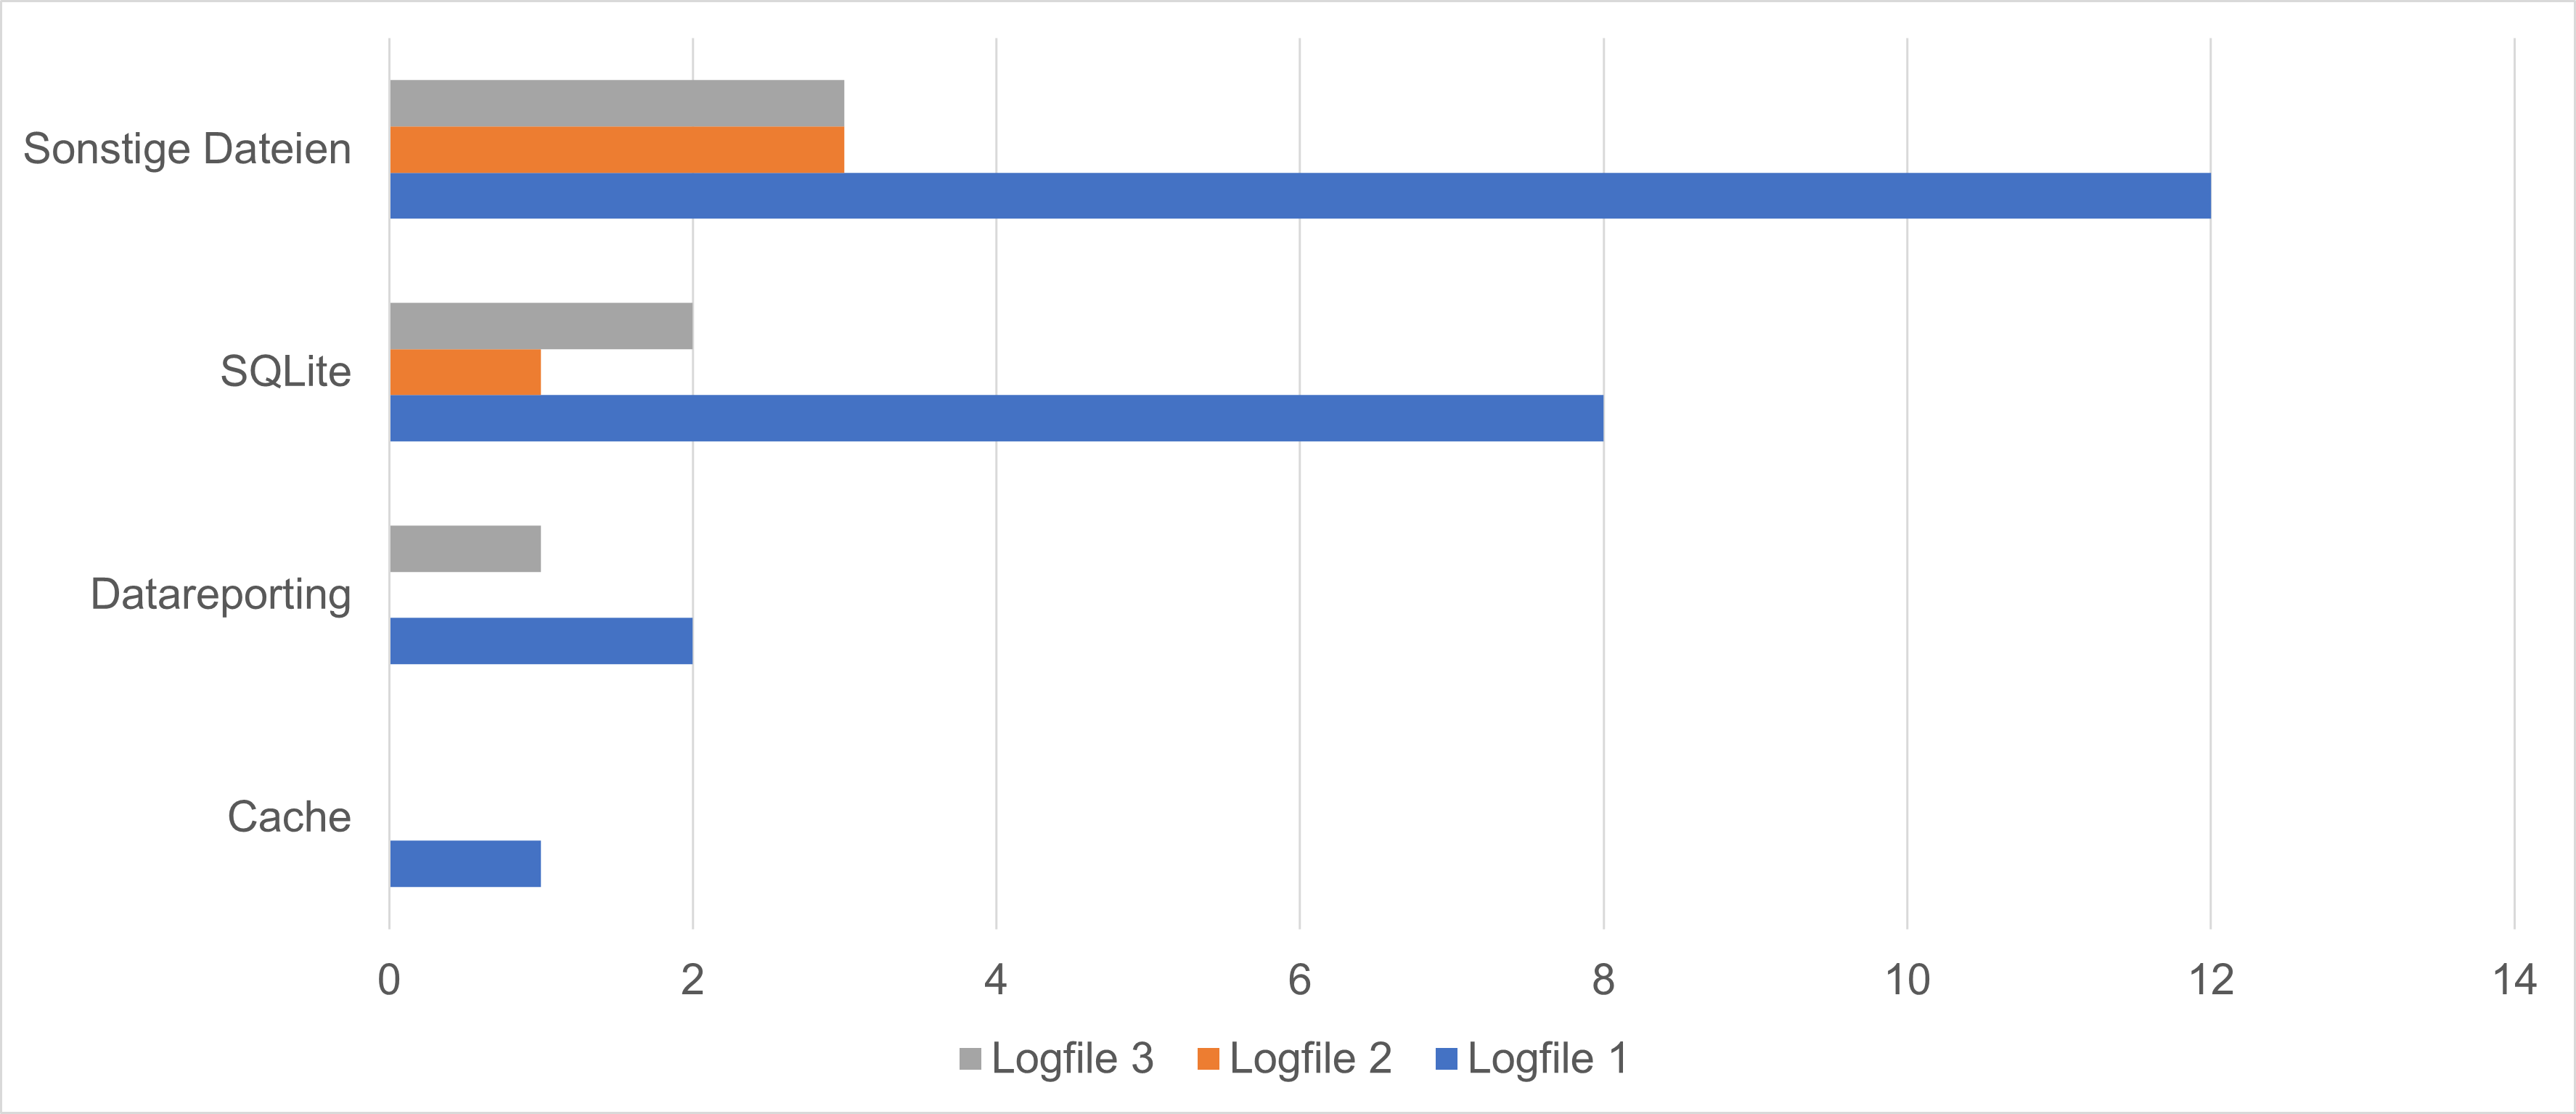
\includegraphics{bilder/tor-bar-chart-logfile1vs2cs3.png}}}
		\label{chart:final-criteria}  
		\caption{Comparison of found PB artifacts between RAM Dumps}
	\end{figure}

%Literatur:
%	o no traces were found in “common locations” \cite{Montasari.2015}
%		>  “places.sqlite”, “webappsstore. sqlite”, “sessionstore.bak”, “search.json” and “nssckbi.dll”
%	o	Safebrowsing: Alle Dateien in /safebrowsing-updating/ nicht relevant. Dort nur .vlpset und .sbstore Dateien. Speichern 256-Bit Hash von URLs, die auf SafeSearch Blacklist stehen 
%	o	Cache-Dateien: drei Caches: startupCache, jumpListCache (beide enthalten Binärdateien ohne Browsing Artefakte) und cache2 (können mit MozillaCacheView untersucht werden, enthalten keine Browsing Artefakte)
%	o	SQLite Datenbanken: Sqlite Dateien erst ohne WAL Dateien untersuchen, Danach mit sqlite3 Konsole: WAL in Datenbank schreiben mit: PRAGMA wal\_checkpoint; places.sqlite besonders relevant, da dort Browser in public Modus Browsing URLs verwaltet (Am besten hier vergleich mit Public Browsing machen)	
%		> \cite{Fayyad.2021} for Mozilla Firefox, 7 database files were recovered: cookies.sqlite-shm, places.sqlite-shm, prefs.js etc.
%		> \cite{Muir.2019} The two SQLite databases used by Firefox to track cookies and history (cookies.sqlite und places.sqlite) were both recoverable from the file system after deletion	
%		Ergebnisse stehen im Gegensatz zu \cite{Hedberg.2013} :
%			o	Chrome und Firefox: Einträge in places.sqlite + history.sqlite DB gefunden während PB! (Noch aktuell??)
%		Sonderfall: SQlite DB-Crash \cite{Hedberg.2013}
%			> WAL Files/Journal Files bei Crash gefunden -> Kann genutzt werden um zu beweisen, dass privater Browser genutzt wurde
%			> Daher: WAL Rollback mit sqlite3	
%	o	Jsonlz4 \& balkz4: Enthalten komprimierte Firefox-Sessions, jsonlz4 Dateien können mit Tool "entkomprimiert" werden: https://www.jeffersonscher.com/ffu/scrounger.html

\subsection*{Uncommon Locations}
			Nachfolgend werden die Analyseergebnisse der Firefox Uncommon Locations beschrieben.
			Wie in Kapitel X erläutert, wird im Gegensatz zu Common Locations die Suchrichtung umgekehrt und es werden alle gesammelten Daten nach einem spezifischen PB Artefakt durchsucht.
			Somit benötigt ein Forensiker kein Wissen über das Browserverhalten. Stattdessen wird sich auf die Vollständigkeit der Funktionen von Forensik-Tools verlassen. Im Rahmen dieses Versuchs werden die Tools Autopsy und Volatility verwendet.

\subsubsection*{Analyse mit Autopsy}

			Bei den Common Locations in Kapitel X wird Autopsy nur zur Dateiextraktion genutzt. Im Falle der Uncommon Locations dient Autopsy als forensisches Werkzeug zur Datenanalyse.

Bei White-Box Analyse/Common Locations: Autopsy nur zur Dateiextraktion genutzt, hier: als konkretes forensisches Werkzeug

Stichwortsuche:
- In allen Snapshots keine Treffer (auch innerhalb \$Carved)
- TODO: Pagefile gefunden?

Von Autopsy automatisch indexierte Dateien: 
In allen Fällen: keine Dateien gelöscht, nur über Zeitraum der Snapshots neue dazugekommen
- Web Bookmarks:
	\begin{figure}[h!]
		\centerline{\resizebox{\linewidth}{!}{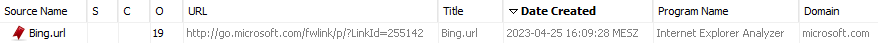
\includegraphics{bilder/cfv_tor_autopsy_web_bookmarks.png}}}
		\label{chart:final-criteria}  
		\caption{Autopsy Web Bookmarks}
	\end{figure}
	Snapshot 1:
		> Bing.url (Unter C:/User/Forensik/Favorites/Links) enthält Bing Startseite
	Snapshot 2:
		> unverändert zu 1
	Snapshot 3-1:
		> unverändert zu 2
	Snapshot 3-2:	
		> unverändert zu 3-1
	Snapshot 4:
		> unverändert zu 3-2
- Web Cookies:
	\begin{figure}[h!]
		\centerline{\resizebox{\linewidth}{!}{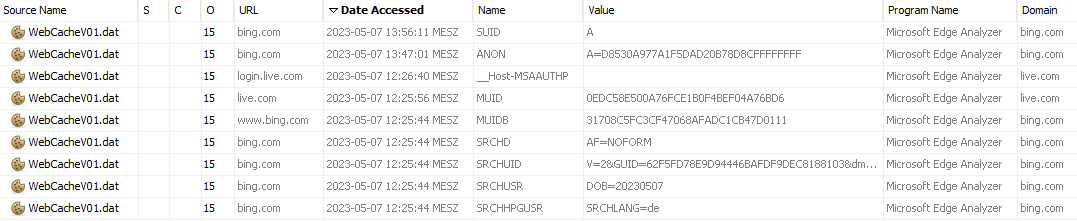
\includegraphics{bilder/cfv_tor_autopsy_web_cookies.png}}}
		\label{chart:final-criteria}  
		\caption{Autopsy Web Cookies}
	\end{figure}
	Snapshot 1:
		> 9 Einträge in WebCacheV01.dat (= DB des Internet Explorers zum speichern von Browserdaten): Cookies für bing.com und live.com (= outlook)
	Snapshot 2:
		> unverändert zu 1
	Snapshot 3-1:
		> unverändert zu 2
	Snapshot 3-2:
		> unverändert zu 3-1
	Snapshot 4:
		> unverändert zu 3-2
- Web History:
	\begin{figure}[h!]
		\centerline{\resizebox{\linewidth}{!}{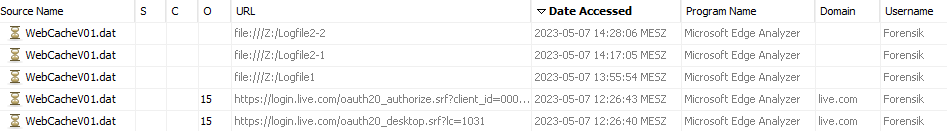
\includegraphics{bilder/cfv_tor_autopsy_web_history.png}}}
		\label{chart:final-criteria}  
		\caption{Autopsy Web History}
	\end{figure}
	Snapshot 1:
		> 2 Einträge in WebCacheV01.dat:
			- 2x live.com (= outlook)
	Snapshot 2:
		> 1 neuer Einträge in WebCacheV01.dat:
			- file:///Z:/Logfile\_1 (= Process Monitor Logfile, die in shared-Folder geladen wurde) -> Erklärung?
	Snapshot 3-1:
		> 1 neuer Eintrag in WebCacheV01.dat:
			- file:///Z:/Logfile\_2-1 (= Process Monitor Logfile, die in shared-Folder geladen wurde) -> Erklärung?
	Snapshot 3-2:
		> 1 neuer Eintrag in WebCacheV01.dat:
			- file:///Z:/Logfile\_2-2 (= Process Monitor Logfile, die in shared-Folder geladen wurde) -> Erklärung?
	Snapshot 4:
		> unverändert zu 3-2
- Web Categories:
	\begin{figure}[h!]
		\centerline{\resizebox{\linewidth}{!}{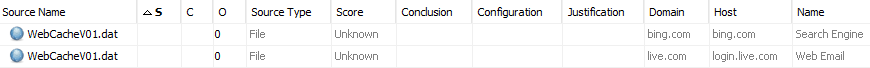
\includegraphics{bilder/cfv_tor_autopsy_web_categories.png}}}
		\label{chart:final-criteria}  
		\caption{Autopsy Web Categories}
	\end{figure}
	Snapshot 1:
		> 2x WebCacheV01.dat aufgelistet => Mit HxD untersucht, keine PB Artefakte
	Snapshot 2:
		> unverändert zu 2
	Snapshot 3-1:
		> unverändert zu 3
	Snapshot 3-2:
		> unverändert zu 3-1
	Snapshot 4:
		> unverändert zu 3-2
		
Zusammenfassung:
- keine PB Artefakte
- Keine neuen Erkenntnisse vgl. mit intensiver Analyse mittels Process Monitor in Kapitel X
- .onion URL Einträge in places.sql nicht erkannt

%Literatur:
%	o	Autopsy Keywortsuche: 
%		>	In alles Snapshots ergebnislos (keine Keyword-Hits
%		-->	In Literatur: Autoren fanden Ergebnisse in pagefile.sys 
%			> Autopsy: websites and some of the keywords found in hidden file called “pagefile.sys” \cite{Mahlous.2020}
%			o \cite{Montasari.2015} traces were found in: 
%				> However, on investigating the “pagefile.sys”, some entries were discovered
%				> Using the “data carving” technique, profile picture was recovered
%			o \cite{Said.2011} 
%				> Examining pagefile.sys showed some positive hits 			
%		--> Evtl. hier zeigen, was gefunden werden kann, wenn RAM reduziert
%		--> Aber auf Problem hinweisen, dass gefundener String in pagefile nicht direkt Browser zugeordnet werden kann
%		> \cite{Gabet.2018}	Firefox only produced three recoverable artefacts as reported by both tools (FTK, Autopsy) --> Artefakte werden nicht genannt!
%		> \cite{Muir.2019} Autopsy Keyword Suche nach Suchbegriffen: unallocated space
%		> Autopsy Carving Module (\$Carved): \cite{Muir.2019}
%			•	When searching for the string ’clot’ from the browsing protocol, six .dll, .edb and .reg files were discovered in unallocated space.
%			•	Further searching of unallocated space uncovered references to the Tor installation directory and the obfs4 bridging IP addresses
%			•	browsing data found in NTUSER.DAT was also replicated in unallocated space.
%	o	Autopsy PlugIns:
%		>	*** TODO: Hier Liste mit PlugIns ***

\subsubsection*{Analyse mit Volatility}
			Nachdem die Firefox Festplattenabbilder als Uncommon Location mit Autopsy untersucht wurden, werden nachfolgend die Analyseergebnisse des RAMs als Uncommon Location beschrieben. 
			Dazu wurde eine Stringsuche im gesamten RAM nach PB Artefakten durchgeführt.
			Wie in Kapitel X ausführlich beschrieben muss ein gefundener String eindeutig einem Browser zugeordnet werden können. 
			
			Deshalb wurde dazu das Volatility PlugIn "Yarascan" verwendet, ein Werkzeug um nach bestimmten Mustern im RAM zu suchen. Dazu wurden die in Tabelle X aufgeführten Yara-Regeln verwendet.
			Wie in Kapitel Methodik (TODO!) beschrieben, wird davon ausgehend das PlugIn "pslist" verwendet, um den Prozessnamen anhand PID zu identifizieren.
			Die Ergebnisse dieser Stringsuche sind nachfolgend nach Kategorie geordnet.


Vorgehen: Siehe "Methodik" Kapitel
	- Ausgangslage: Volatility Yarascan Treffer
	- Für jeden Treffer: virtueller Offset des Strings, PID, getriggerte Yararule, getriggerte Yara Component z(= Variablenname des gesuchten Strings), gefundener String
	- Neue Spalte: "Prozessname" -> zu jeder PID Prozessnamen
	- Ergebnisse Aufbereitet nach folgendem Schema:
		> Für jeden RAM Dump
		> Für jede Yararule
		> Für jede Component
		> Filter: Prozessname = Firefox -> Anzahl zählen
		> Filter: Prozessname = Alle Prozesse außer Firefox -> Anzahl zählen

Wie bei Firefox: HTML Artefakte wurden in keinem RAM Dump gefunden => Nicht aufgeführt

Yararule "Keyword":
	\begin{figure}[h!]
		\centerline{\resizebox{\linewidth}{!}{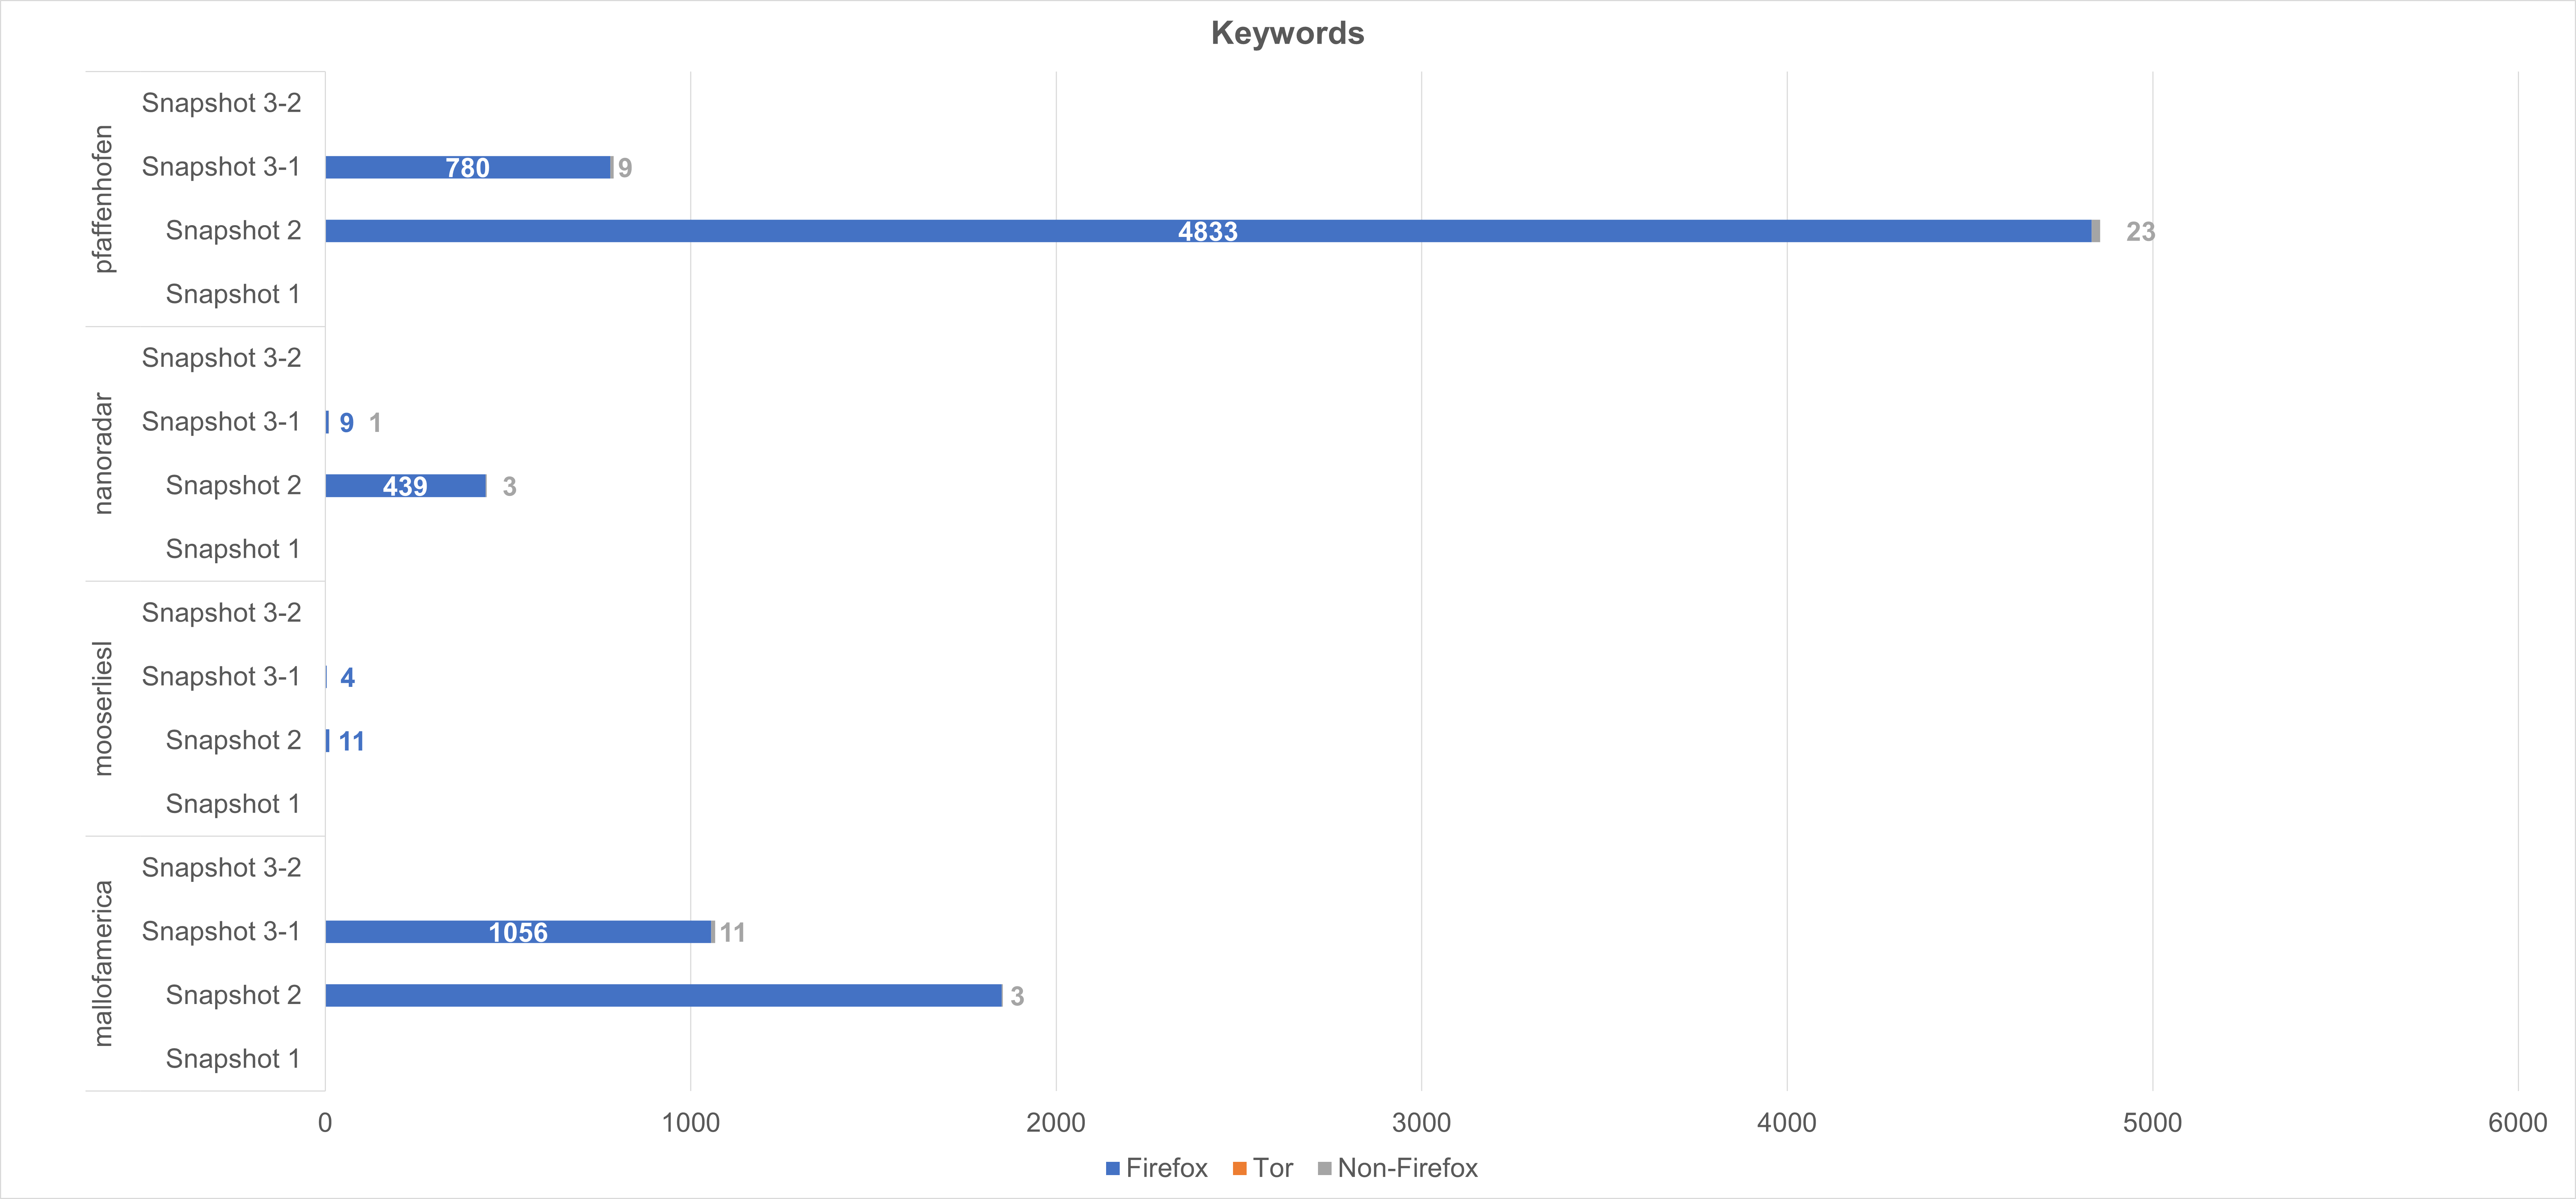
\includegraphics{bilder/volatility/tor/keywords.png}}}
		\label{chart:final-criteria}  
		\caption{Keywords}
	\end{figure}
	Analyse:
		> Ausschließlich in RAM Dump 2 und RAM Dump 3-1 Keyword Artefakte gefunden
		> In RAM Dump 3-1 bei jedem Keyword deutlich weniger Artefakte als in RAM Dump 2 => Identitäts-Reset reduziert Keyword Artefakte deutlich
		> Hauptsächlich in Firefox Prozess, kein Artefakt in Tor.exe Prozess
		> Mit 4833 Artefakten in RAM Dump 2 am häufigsten "pfaffenhofen" vertreten. Vermutung: Evtl. weil Google Maps viele zusätzliche Artefakte lädt. 
		> Nach Schließen von Tor Browser: keine Keyword Artefakte mehr in RAM
		
Yararule "URL":
	\begin{figure}[h!]
		\centerline{\resizebox{\linewidth}{!}{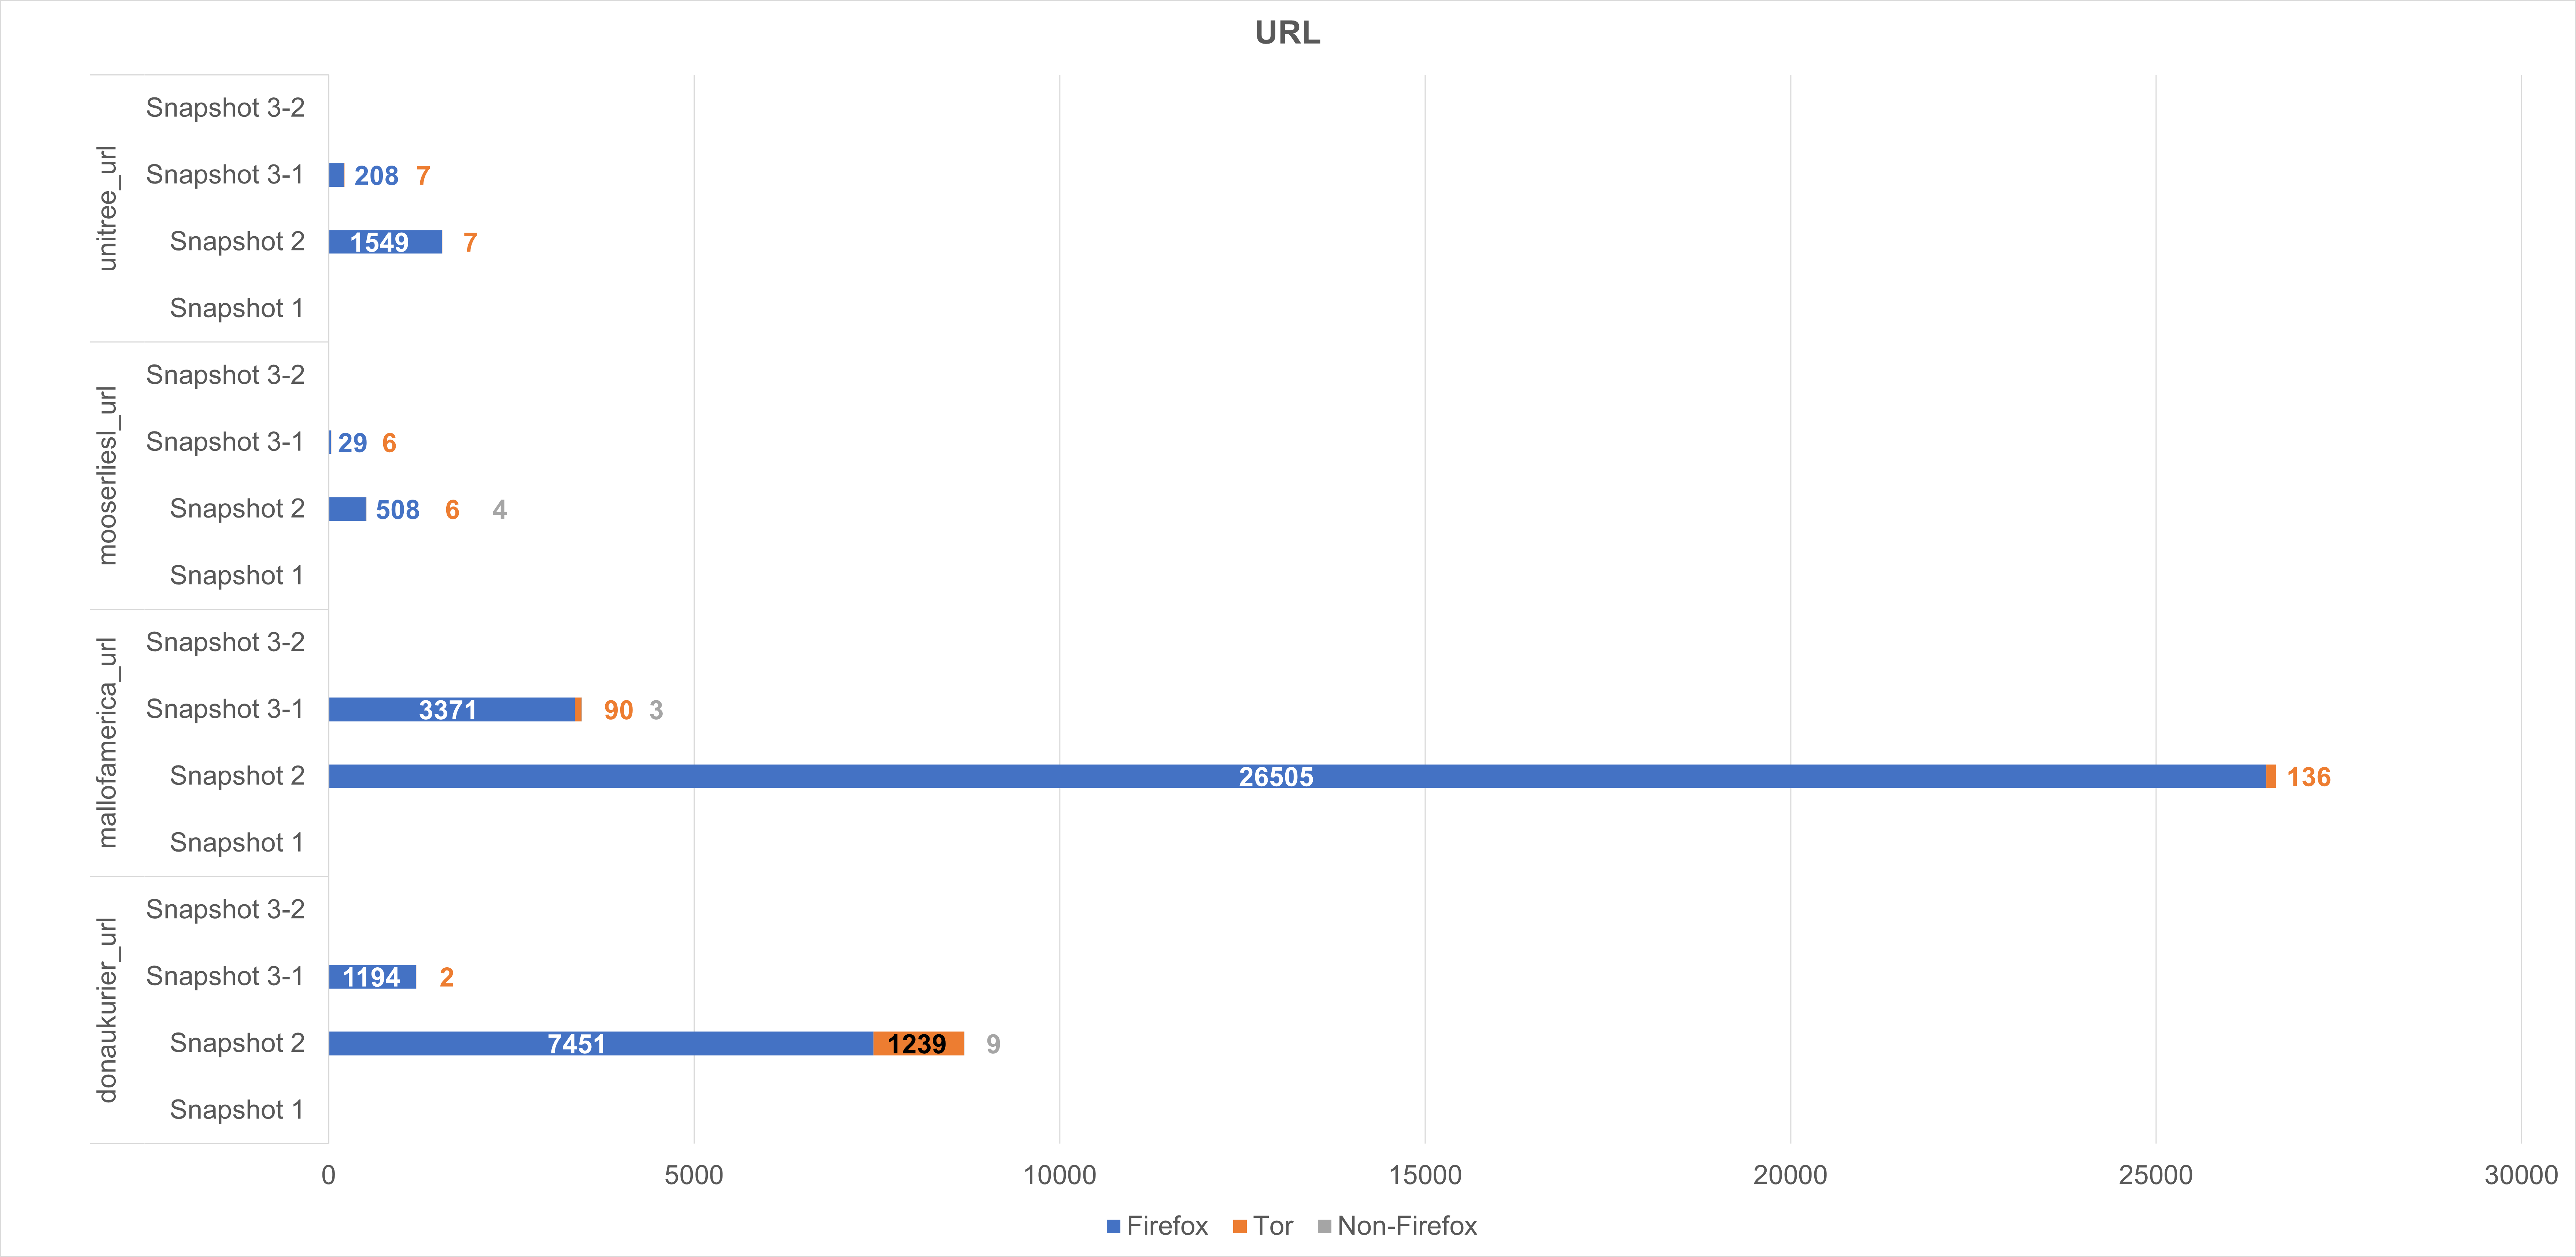
\includegraphics{bilder/volatility/tor/url.png}}}
		\label{chart:final-criteria}  
		\caption{URL}
	\end{figure}
	Analyse:
		> Wie bei Yararule "Keyword": Ausschließlich in RAM Dump 2 und RAM Dump 3-1 Keyword Artefakte gefunden
		> In RAM Dump 3-1 bei jedem Keyword deutlich weniger Artefakte als in RAM Dump 2 => Identitäts-Reset reduziert URL Artefakte deutlich
		> Hauptsächlich in Firefox Prozess, danach am häufigsten Tor.exe Prozess und am wenigsten Artefakte in anderen Prozessen
		> Bemerkenswert: "mallofamerica.com" ist mit 26.505 mal in RAM Dump 2 am häufigsten als Artefakt gefunden worden. Vergleich: "mooserliesl.de" wurde nur 508 mal in RAM Dump 2 gefunden
		> Nach Schließen von Tor Browser: keine URL Artefakte mehr in RAM
		
		> TODO: DNSCache?

Yararule "Mail":
	\begin{figure}[h!]
		\centerline{\resizebox{\linewidth}{!}{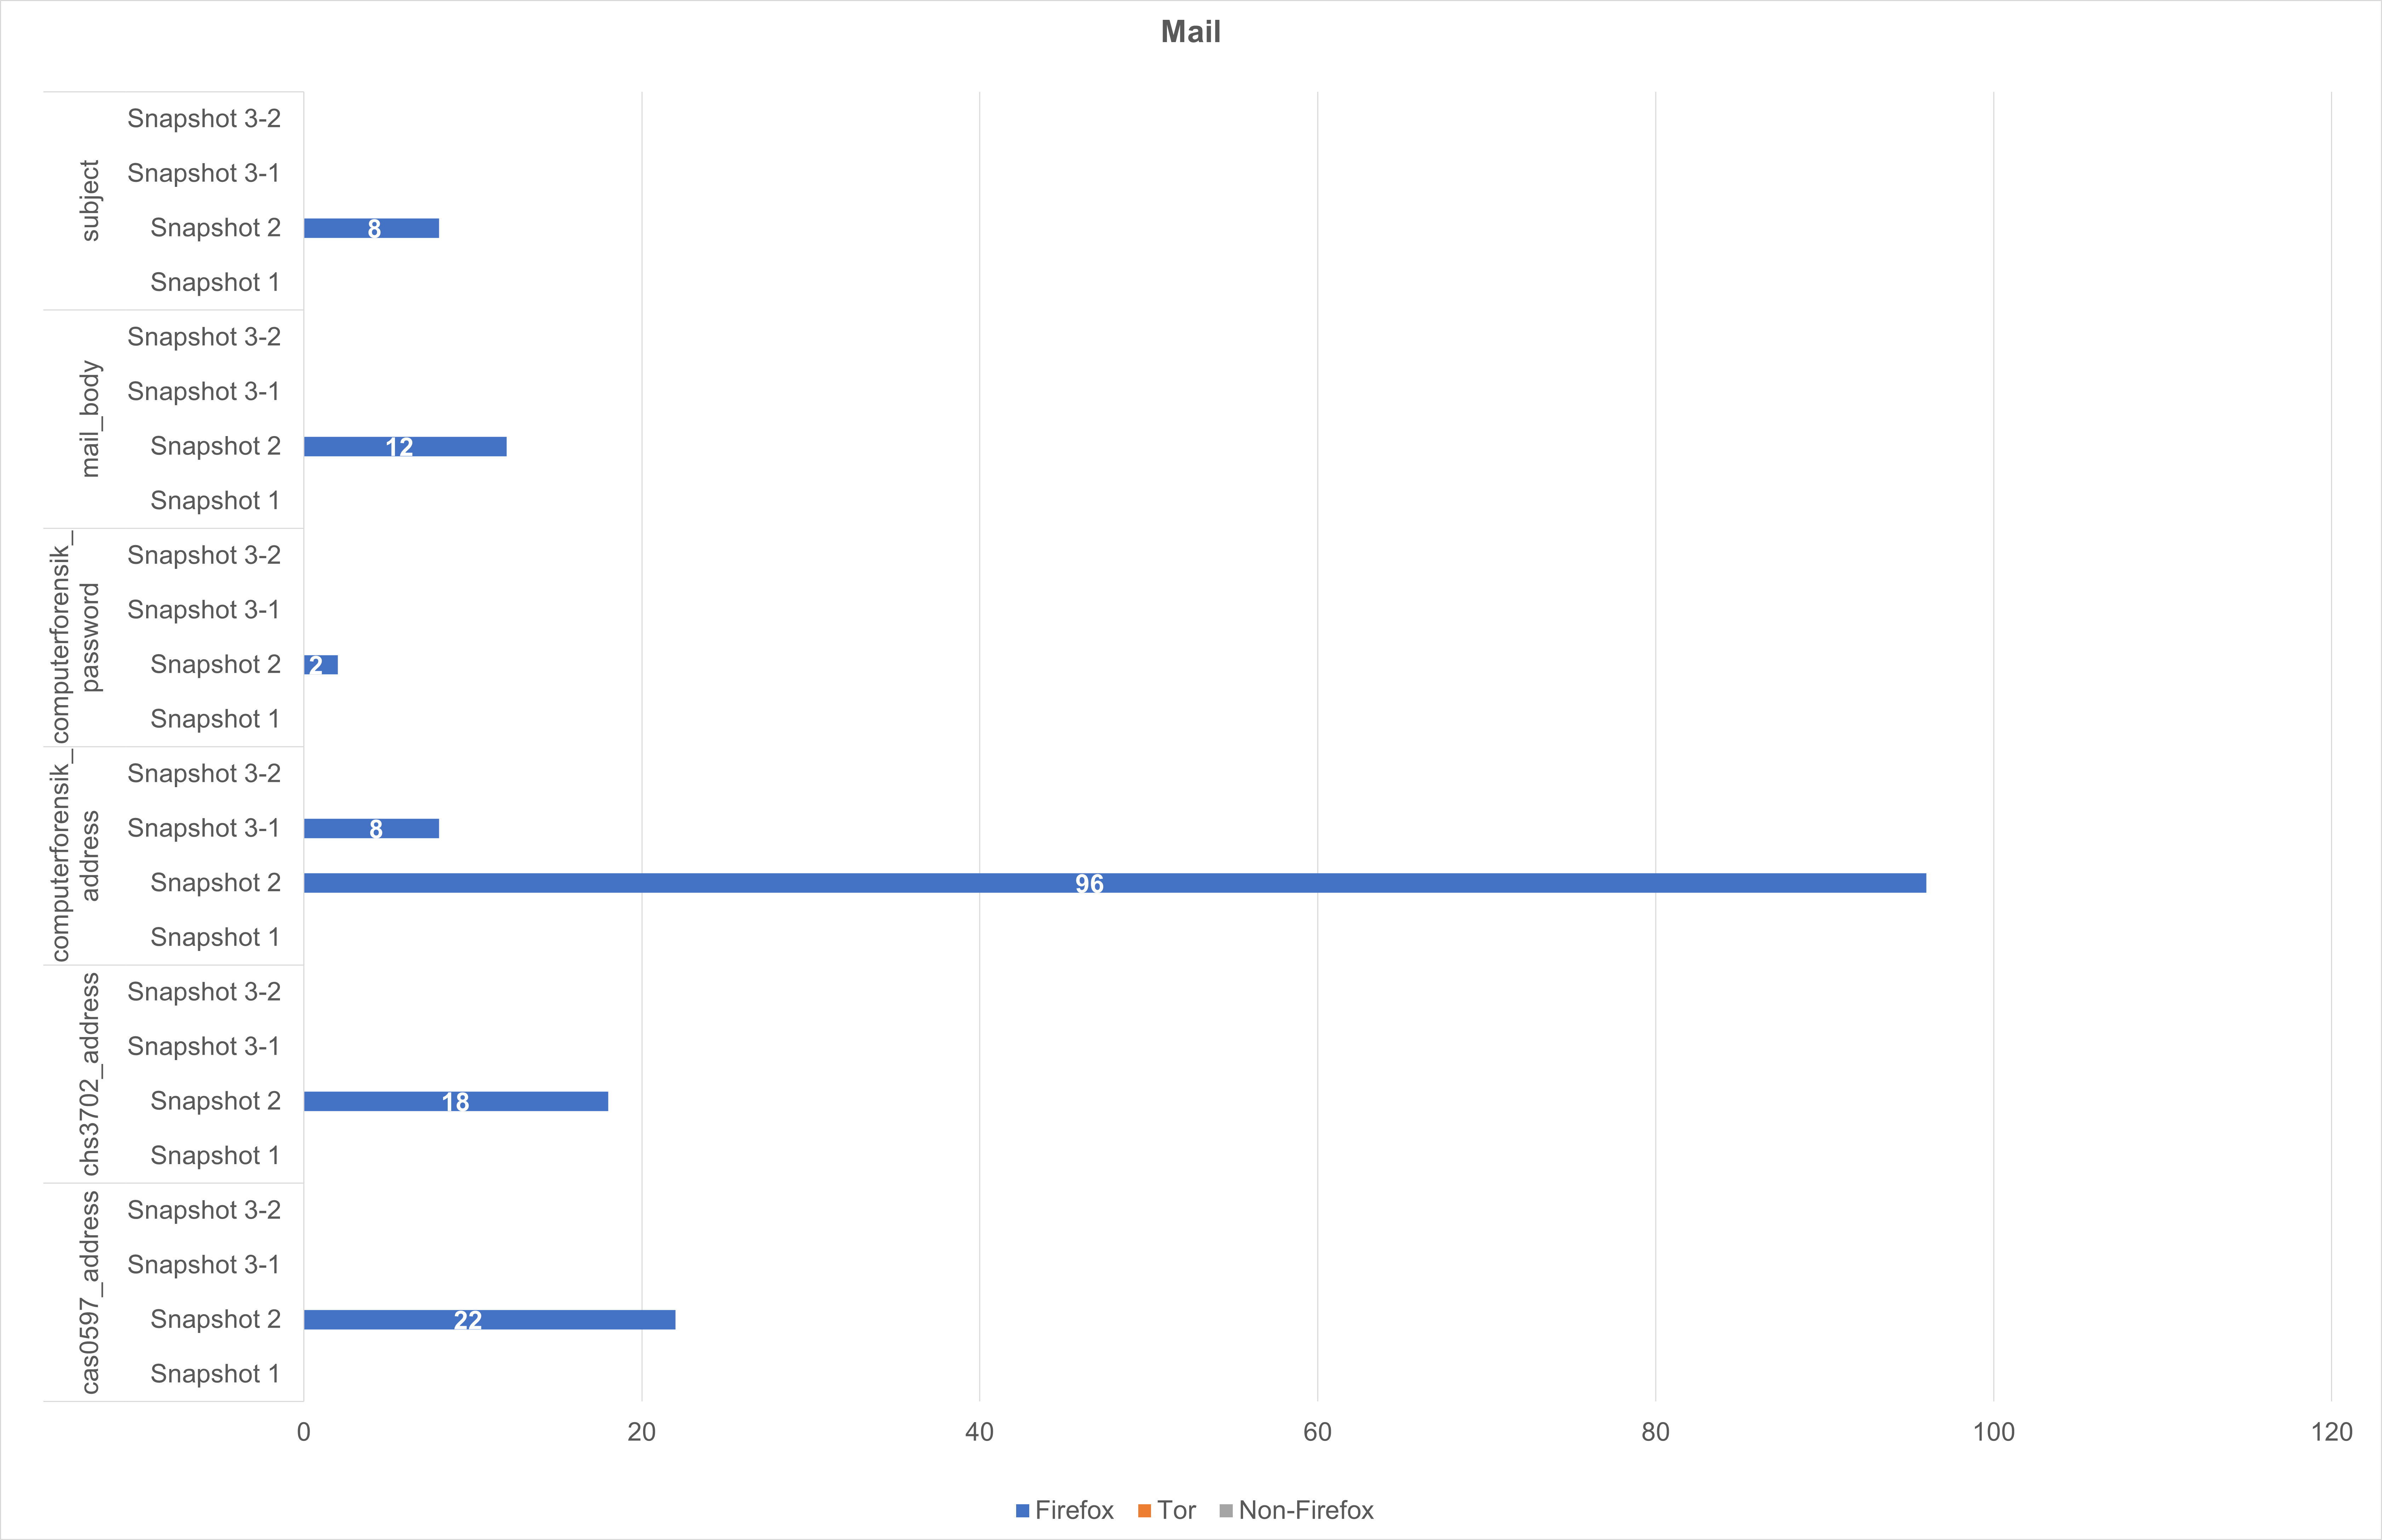
\includegraphics{bilder/volatility/tor/mail.png}}}
		\label{chart:final-criteria}  
		\caption{Mail}
	\end{figure}
	Analyse:
		> Alle Mail Artefakte gefunden
		> Artefakte ausschließlich in Firefox Prozess gefunden
		> Artefakte fast ausschließlich in RAM Dump 2 Mail gefunden
		> Nur die Absenderadresse "computerforensikvl@gmail.com" wurde nach Identitäts-Reset in RAM Dump 3-1 gefunden
		> Absenderadresse ist häufigstes Mail Artefakt
		> Bemerkenswert: Passwort wurde 2x als Klartext im RAM gefunden!
			String Kontext:
				Offsets:		PIDs:
				0xb9ce29180c8	7420
				0x2859f4ffd4e0	7420
				0x24083b41858	8424
				0x240840e5b08	8424
				
Yararule "Image":
	\begin{figure}[h!]
		\centerline{\resizebox{\linewidth}{!}{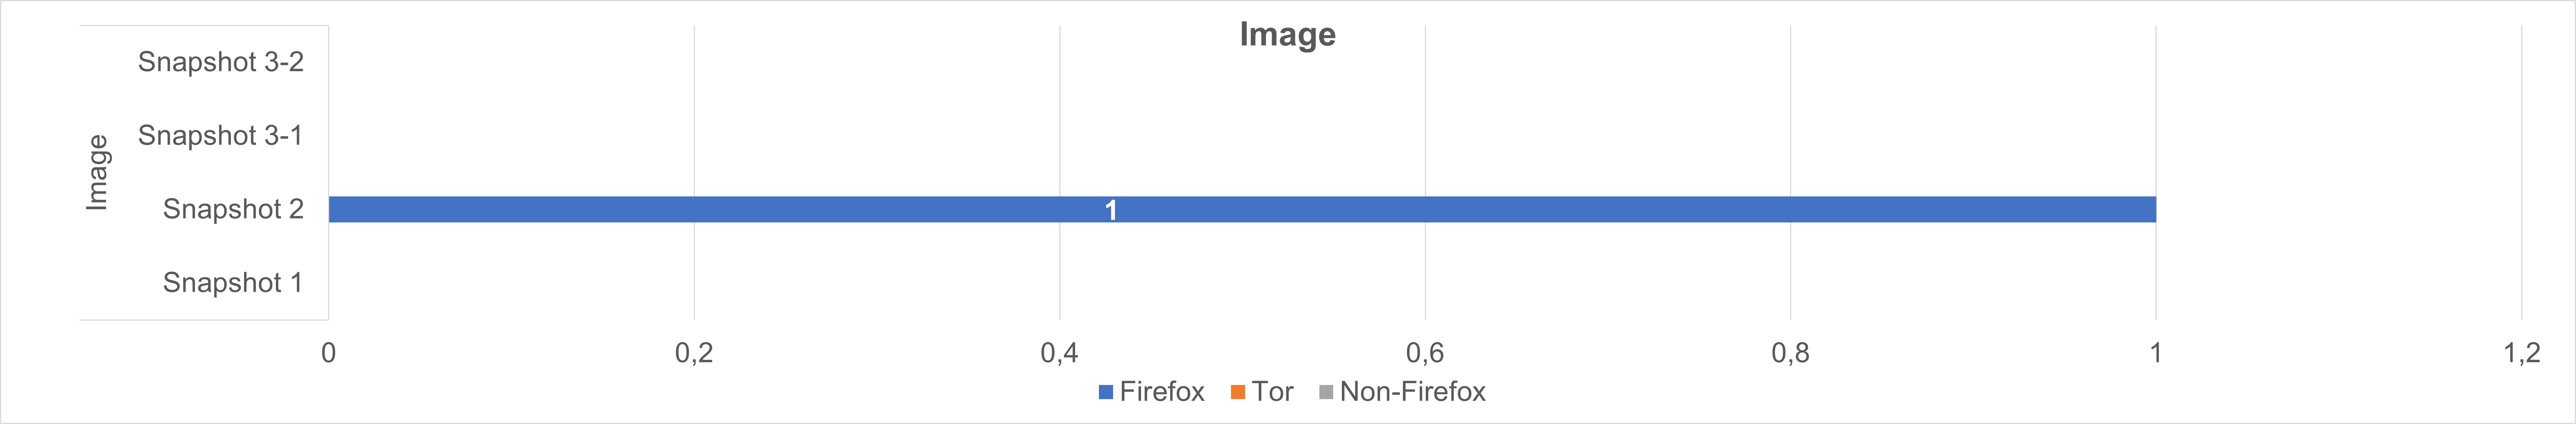
\includegraphics{bilder/volatility/tor/image.png}}}
		\label{chart:final-criteria}  
		\caption{Image}
	\end{figure}
	Analyse:
		> Hex-Wert von Donaukurier Bild wurde ein einzigees mal im 2. RAM Dump in einem Firefox Prozess gefunden
	

Zusammenfassung = Stacked Bar Chart:
\begin{figure}[h!]
	\centerline{\resizebox{\linewidth}{!}{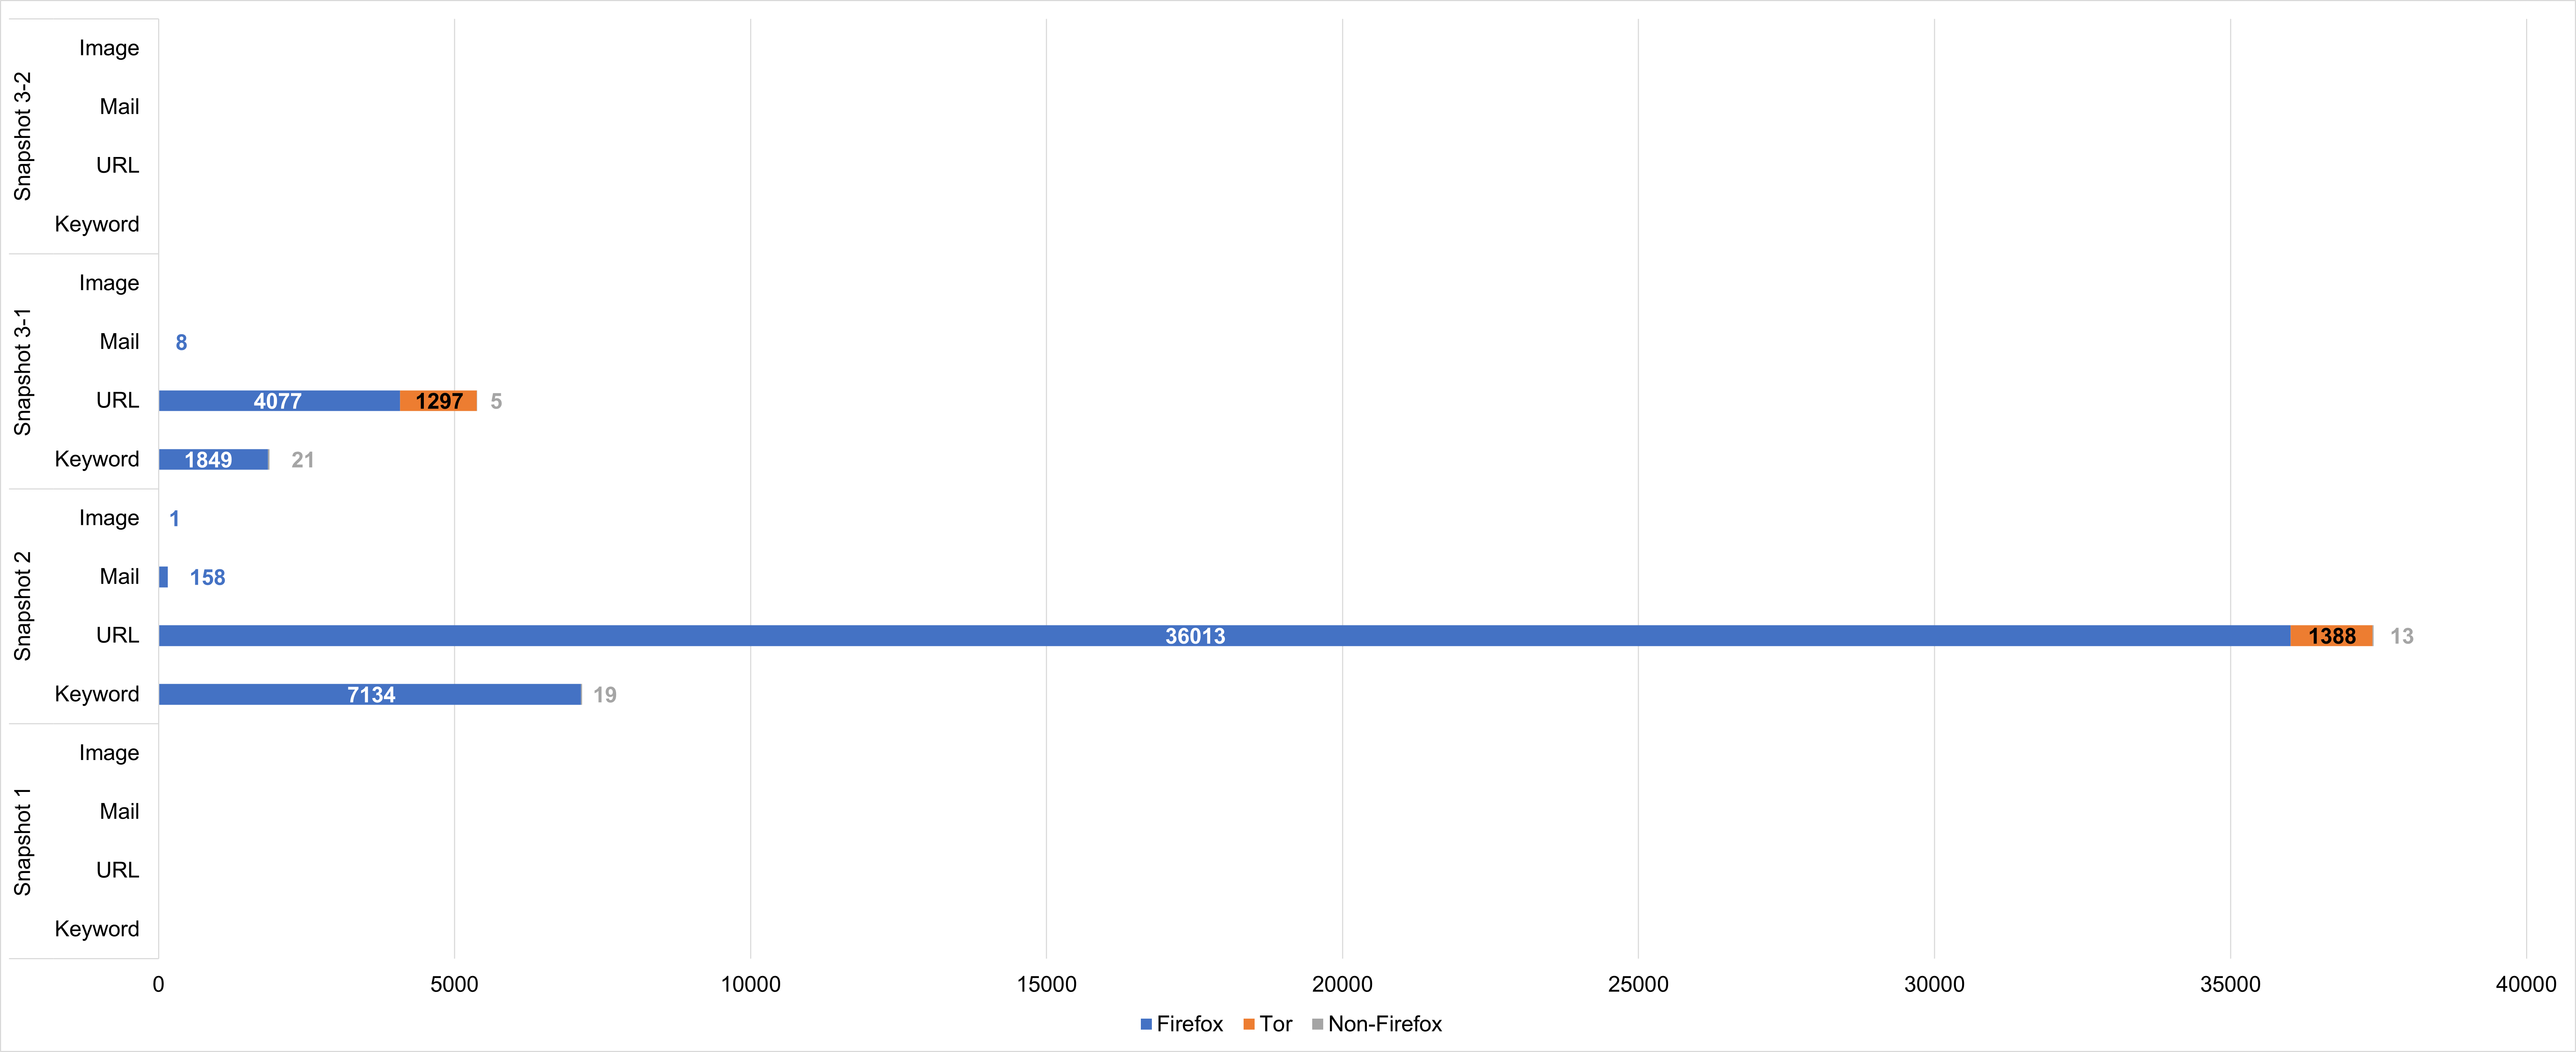
\includegraphics{bilder/volatility/tor/summary.png}}}
	\label{chart:final-criteria}  
	\caption{Summary}
\end{figure}
- PB Artefakte ausschließlich in RAM Dump 2 und 3-1 gefunden
- Nach Identitäts-Reset deutlich weniger Artefakte in vorhanden
- Am meisten URL-Artefakte gefunden, wobei mallofamerica.com dominant 
- HTML Artefakte wurden in keinem RAM Dump gefunden


TODO: Kreisdiagramme/Balkendiagramme mit Gesamtzahl an (Non-)Firefox Yarascan-Treffer erst im Vergleich mit Tor

Literatur:
%o Autopsy: \cite{Muir.2019}
%	•	Configuration files, downloaded files, and browserrelated data are recoverable from the file system.
%	•	Significant data-leakage from the browsing session occurred: HTTP header information, titles of web pages and an instance of a URL were found in registry files, system files, and unallocated space.
%o RAM-Analyse nach \cite{Muir.2019}:
%	•	Live-Analyse identifiziert auch nach dem Schließen und Deinstallieren des Browsers und Abmelden des Benutzers Spuren von Tor-Prozessen, einschließlich des absoluten Pfads zur Browser-Executable, des Benutzernamens und des Geräts, von dem es ausgeführt wurde.
%	•	The data-leakage contained the German word for ’search’ in reference to a Google search. This hints at the locale of the Tor server used to exit the network (exit relay).
%
%o RAM-Analyse nach \cite{Hariharan.2022}:
%	o	process was found to be firefox.exe
%	o	pslist and pstree: parent process was shown 
%	o	Belkasoft Ram Capturer: retrieve information about facebook
%	o	Cmdline: file path of the browser “E:/TorBrowser/Browser/firefox.exe” + name of process tor.exe and firefox.exe
%	o	Dlllist: DLL files of the executable files were not captured
%	o	Netscan: tor.exe + obfs4proxy.exe -> showed “LISTENING” connections to nonstandardized ports as output.
%	Yarascan: was able to retrieve all the browsing sessions
%o RAM-Analyse nach \cite{Sajan.2021} mit Volatility
%	•	process list extracted from the memory
%	•	registry hives been extracted from the memory dump
%	•	threads were extracted: “D:/VolatilityWorkbench/volatility.exe”–plugins=”D:/VolatilityWorkbench/profiles” pslistfilename =”C:/Users/username/Desktop/tor.raw” –profile=Win10x64 17763 –kdbg=0xf807606ac5e0
%	•	Handles: resources used by the process 5672
%	•	Dlls: These dlls can be found from prefetch file --> Can be found in “prefetch” file -> Analyzed with “winprefetchview”
%	•	Places.sqlite: SQLite viewer has been used to recover bookmarks and frequently visited sites even after uninstalling the application
%	•	Visited Websites: Using keyword search in Dump’s Hex
%
%o Registry:
%	> Shellactivites (siehe Firefox) \cite{Muir.2019}: instance of a URL were found in registry file
%	> \cite{Nelson.2020} The userassist key is located in the NTUSER.dat hive of the
%		 -> Registry and indicates the execution path of the program, as well as the number of times the program was executed 

\subsection*{Registry}

			Die Analyse der Registry zählt gemäß Methodik in Kapitel X sowohl zu den Common als auch Uncommon Locations 

\subsubsection*{Process Monitor SetValue Operations}

			Als Teil der Common Locations werden für Firefox alle Registry "SetValue" Schreiboperationen der beiden Process Monitor Logfiles untersucht.

> Process Monitor: SetValue Operationen von Browser 
	Kategorien Registry Keys: Analog zu Firefox
	1) PreXULSkeletonUISettings:
		> Prefix: Absoluter Installationspfad von Firefox
		> Skeleton UI Einstellungen von Firefox % https://itigic.com/skeleton-ui-new-firefox-interface-to-start-up-much-faster/#google_vignette
			Definition:
				> Der "PreXULSkeletonUISettings" Registry Key enthielt Einstellungen für die Benutzeroberfläche (UI) des Firefox-Browsers, insbesondere für das sogenannte "Skeleton UI". Das Skeleton UI ist eine vereinfachte Benutzeroberfläche, die während des Ladens des Browsers angezeigt wird, bevor die vollständige Benutzeroberfläche geladen ist. Es besteht aus grundlegenden Steuerelementen und Elementen, die dem Benutzer die Interaktion ermöglichen, während der Rest der Benutzeroberfläche noch geladen wird.
				> Der "PreXULSkeletonUISettings"-Schlüssel enthielt Konfigurationsoptionen wie Farben, Positionen und andere Einstellungen für das Skeleton UI. Durch das Bearbeiten dieses Schlüssels konnten Benutzer die Darstellung des Skeleton UI anpassen. Es ist jedoch wichtig zu beachten, dass das Ändern der Registrierungseinträge ein fortgeschrittenes Verfahren ist und Fehler zu Problemen mit dem Browser führen kann.
			
		> Struktur der Keys: % HKCU\SOFTWARE\Mozilla\Firefox\PreXULSkeletonUISettings\C:\Program Files\Mozilla Firefox\firefox.exe|<UI Einstellung>
		> Unterschiedliche UI Einstellungen
			- % ScreenX (DWORD)
			- % ScreenY (DWORD)
			- % Width (DWORD)
			- % Height (DWORD)
			- % Maximized (DWORD)
			- % Flags (DWORD)
			- % CssToDevPixelScaling (REG_BINARY)
			- % UrlbarCSSSpan (REG_BINARY)
			- % SearchbarCSSSpan (REG_BINARY)
			- % SpringsCSSSpan (REG_BINARY)
		> keine PB Artefakte unter UI Einstellungen	
	2) Business Activity Monitoring % https://learn.microsoft.com/de-de/biztalk/core/business-activity-monitoring-bam
		> Quelle: % https://notes.qazeer.io/dfir/windows/_artefacts_overview
		> BAM is a mostly undocumented feature that controls the programs executed in the background. DAM is a feature for devices supporting the "Connected Standby" mode (i.e when a device is turned on, but its display will be turned off). As a result, the BAM registry keys will contain data on any devices, while DAM registry keys will only contain data on mobile devices.
		> The BAM registry key contains multiple subkeys under bam\\State\\UserSettings, with one subkey per user, identified with the user SID. While the key is in the SYSTEM registry hive, program executions can thus still be tied to a specific user using this SID.
		> Each user-specific key contains a list of executed programs, with their full path and timestamp of last execution.
		> If a file is deleted, the eventual associated entry in the BAM is deleted as well after the system reboot. Additionally, BAM entries older than 7 days are deleted upon system boot. The BAM thus provides limited information on historic execution of programs
		> No entries are created in the BAM keys for executables on removable media and/or on network shares.
		> Key: %  HKLM\System\CurrentControlSet\Services\bam\State\UserSettings\S-1-5-21-588412547-2749917301-3803556669-1001\\Device\HarddiskVolume2\Program Files\Mozilla Firefox\firefox.exe (REG_BINARY)

Quantitativ: (Diagramme)
	- Stacked Balkendiagramm jeweils für Logfile 1 und Logfile2: Anteil Kategorie 1 bzw.2 an allen Registry-Schreiboperationen
	\begin{figure}[h!]
		\centerline{\resizebox{\linewidth}{!}{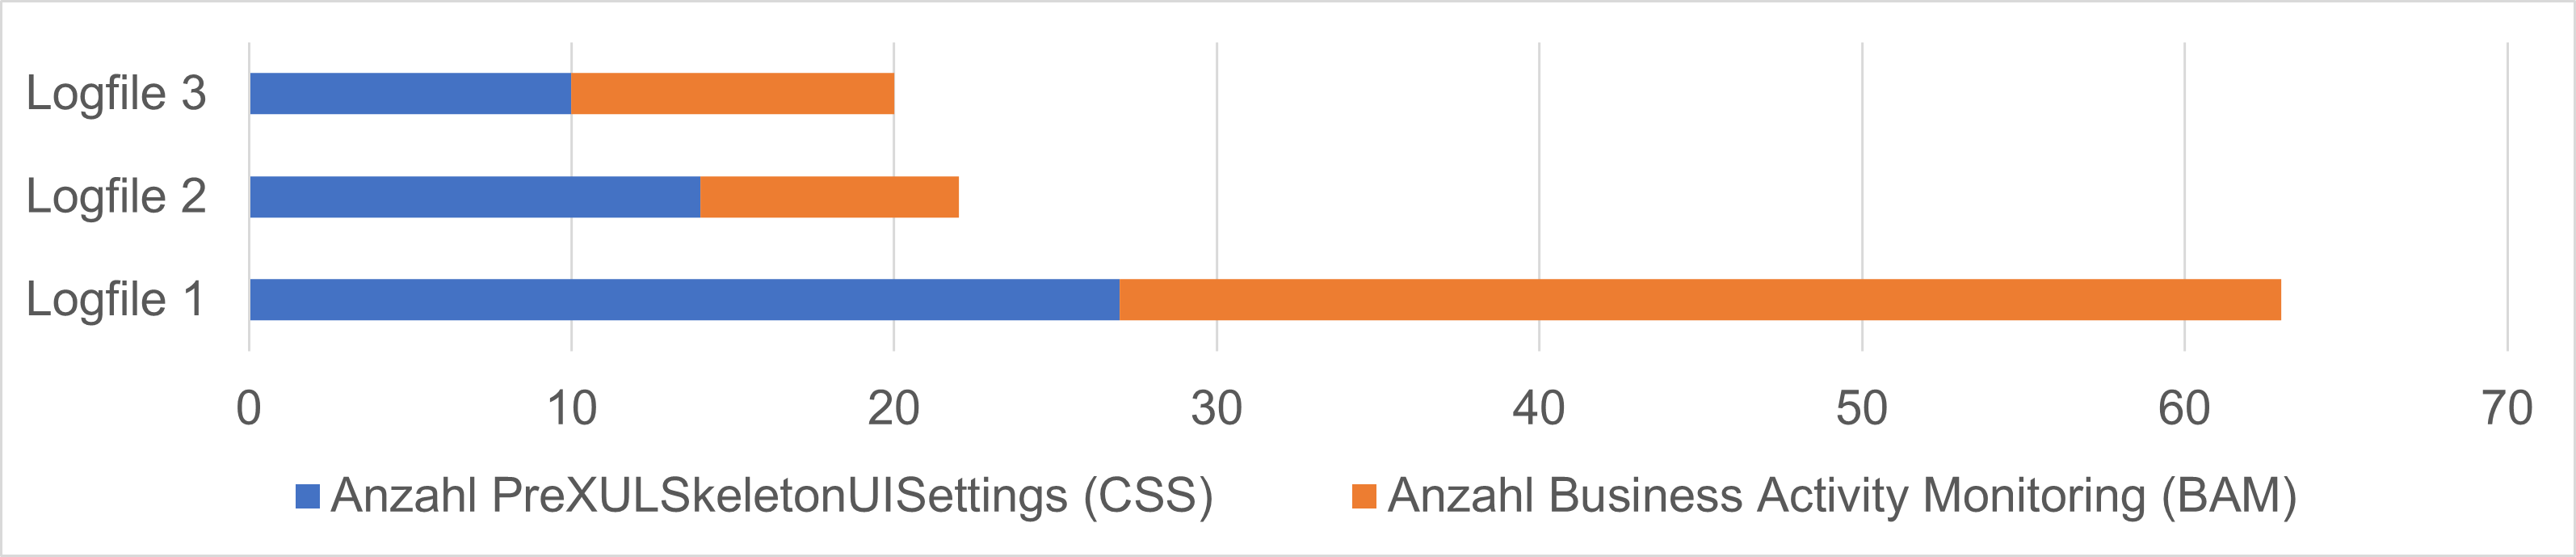
\includegraphics{bilder/tor-registry-stacked-bar-chart.png}}}
		\label{chart:final-criteria}  
		\caption{Comparison of found PB artifacts between RAM Dumps}
	\end{figure}

\subsubsection*{Stringsuche in Registry Hives}

		Gemäß Methodik in Kapitel X wird die Firefox Registry als Uncommon Location behandelt, indem über alle auf der Festplatte vorhandenen Registry Datenbanken, den Registry-Hives, eine Stringsuche durchgeführt wird, ohne die Struktur der Hives zu beachten. 
		Dazu wurden sowohl die System-Hives als auch die User-Hives aus Tabelle X (TODO!) aus jedem Snapshot extrahiert und mithilfe des Registry Explorers nach PB Artefakten durchsucht.
		Dabei wurde in keinem Snapshot in keinem Hive ein PB Artefakt gefunden.
			
		> Stringsuche in Registry Hives mit Registry Explorer (Siehe Liste)
		In allen Hives kein Treffer für alle Suchbegriffe



%Literatur:
%	>	Auf Autor verweisen: angeblich in Shellactivities Ergebnisse. --> Nicht mehr vorhanden in aktueller Version (Verweis auf E-Mail)
%	>	Process Monitor/Regshot zeigen keine relevanten Key-Änderungen
%	> \cite{Muir.2019}: Autopsy Keyword Suche nach Suchbegriffen: Ergebnisse in \%SystemRoot\%Minidump NTUSER.DAT, ntuser.dat.LOG1 (a log of changes to NTUSER.DAT)
%	> Zentral: shellactivites Key:	NTUSER.DAT --> “shellactivities” key \cite{Muir.2019}
%	> \cite{Rochmadi.2017} Detection of registry changes helps to determine what the appropriate plugin is used to search for digital evidence using volatility memory forensic:
%	- RegQueryValue:	HKCU/Software/Microsoft/Windows/CurrentVersion/InternetSettings/Connections/DefaultConnectionSettings
%	- RegCloseValue: 	HKCU/Software/Microsoft/Windows/CurrentVersion/InternetSettings/Connections
%	- IRP\_MJ\_READ: C:/pagefile.sys


\section{Chrome}

\subsection*{Uncommon Locations}

o Autopsy Keyword-Suche: 
	> Chrome and Edge produced five artefacts as reported by both tools. (FTK, Autopsy) \cite{Gabet.2018}
		--> Artefakte werden nicht genannt!
	> only two temporary files (Figure 7) were recovered with Minitool Power Data Recovery but it was a dead end; Location: appdata/…/Chrome/…/ Preferences/RF1533fa.TMP \cite{Fayyad.2021}
	> pagefile.sys file showed no traces at all \cite{Said.2011}
	

\section{Brave}